\documentclass[
	10pt,
	a4paper,
	oneside
]{book}

%%%%%%%%%%%%%%%%%%%%%%%%%%%%%%%%%%%%%%%%%%%%%%%%%%%%%%%%%%%%%%%%%%

\pagestyle{headings}

%%%%%%%%%%%%%%%%%%%%%%%%%%%%%%%%%%%%%%%%%%%%%%%%%%%%%%%%%%%%%%%%%%

% Packages 

\usepackage[utf8]{inputenc}
\usepackage[T1]{fontenc}
\usepackage[
	marginparwidth=2in,
	marginparsep=20pt,
	rmargin=3in
]{geometry}

\usepackage{imakeidx}

\makeindex

\usepackage{amsmath,amssymb,amsthm,mathrsfs}

\usepackage{braket}

\usepackage{hyperref}

\usepackage{theoremref}

\usepackage{framed} % Lets us shade

\usepackage{mathtools}
\mathtoolsset{showonlyrefs} % Only number referenced eq's

\usepackage{enumerate}

\usepackage{tikz}
\usetikzlibrary{matrix}
\usetikzlibrary{decorations.pathmorphing,patterns}
\usetikzlibrary{arrows.meta}
\usetikzlibrary{decorations.pathreplacing,angles,quotes}

\usepackage{pgfkeys}

\usepackage{subcaption}

\usepackage{xcolor}

\usepackage{array}

\usepackage{cancel}

%\usepackage{logicproof}

\usepackage{sidenotes}

\usepackage{glossaries-extra}[symbols]

\usepackage{listings}

\usepackage{venndiagram}

\usepackage{graphicx}
\graphicspath{ {/home/tree/Pictures} }

%%%%%%%%%%%%%%%%%%%%%%%%%%%%%%%%%%%%%%%%%%%%%%%%%%%%%%%%%%%%%%%%%%

% Title Page

\author{Tree}
\title{Cumulative Notes}

%%%%%%%%%%%%%%%%%%%%%%%%%%%%%%%%%%%%%%%%%%%%%%%%%%%%%%%%%%%%%%%%%%

%% New commands

% \nc as new command
\newcommand{\nc}{\newcommand}
\nc{\renc}{\renewcommand}

% \df as emphasized (for definitions)
\nc\df[1]{\textit{\textbf{#1}}}

% Common sets
\nc\integers{\mathbb{Z}}
\nc\zplus{{\mathbb{Z}^+}}
\nc\zminus{{\mathbb{Z}^-}}
\nc\zsubn{{\mathbb{Z}_n}}
\nc\naturals{\mathbb{N}}
\nc\alephnought{{\aleph_0}}
\nc\reals{\mathbb{R}}
\nc\rplus{{\mathbb{R}^+}}
\nc\rationals{\mathbb{Q}}
\nc\complex{\mathbb{C}}

% Matrices
\nc\mmn{\mathcal{M}_{m,n}}
\nc\mn{\mathcal{M}_{n}}
\nc\bij{B_{i,j}}
\nc\bji{B_{j,i}}
\nc\aij{A_{i,j}}
\nc\aji{A_{j,i}}

% Functions
\DeclareMathOperator{\diam}{diam}
\DeclareMathOperator\im{im}
\DeclareMathOperator\supp{supp}
\DeclareMathOperator\lub{lub}
\DeclareMathOperator\glb{glb}
\DeclareMathOperator\lcm{lcm}
\DeclareMathOperator\card{card}
\DeclareMathOperator\chara{char}
\DeclareMathOperator\domain{domain}
\DeclareMathOperator\image{image}
\DeclareMathOperator\range{range}
\DeclareMathOperator\Int{Int}
\DeclareMathOperator\Cl{Cl}

\nc\sumiotoinf{\sum_{i=1}^\infty}
\nc\sumiztoinf{\sum_{i=0}^\infty}
\nc\summotoinf{\sum_{m=1}^\infty}
\nc\summztoinf{\sum_{m=0}^\infty}

\nc\divides{\mid}
\nc\notdivides{\nmid}

\nc\kron{\delta_{ij}}

\nc\ra{\rightarrow}
\nc\Ra{\Rightarrow}
\nc\lra{\leftrightarrow}

% Truth functions
\nc\Hand{H_\land}
\nc\Hor{H_\vee}
\nc\Hra{H_\ra}
\nc\Hlra{H_\lra}
\nc\Hneg{H_\neg}

% Roman numerals
\makeatletter
\nc{\Rn}[1]{\textup{\uppercase\expandafter{\romannumeral#1}}}
\nc{\rn}[1]{\romannumeral #1}
\makeatother

% Physics stuff
\nc\mc[1]{\mathcal{#1}}
\nc\ms[1]{\mathscr{#1}}
\nc\bt[1]{\textbf{#1}}
\nc\eqcl[1]{\bt{#1}^\circ}
\nc\V{\ket{V}}
\nc\W{\ket{W}}
\nc\vecsp{\mathbb{V}}
\nc\Axa{\bt{A}_\bt{x}[\bt{a}]}
\nc\Axi{\bt{A}_\bt{x}[\bt{i}]}
\nc\Bxa{\bt{B}_\bt{x}[\bt{a}]}
\nc\Bxi{\bt{B}_\bt{x}[\bt{i}]}
\nc\bxa{\bt{b}_\bt{x}[\bt{a}]}
\nc\nms[1]{#1_1, \dots, #1_n}
\nc\nbts[1]{\bt{#1}_1, \dots, \bt{#1}_n}

% Logic
\nc\propax{\neg \bt{A} \vee \bt{A}}
\nc\subax{\bt{A}_\bt{x} [\bt{a}] \ra \exists \bt{x} \bt{A}}
\nc\idax{\bt{x} = \bt{x}}
\nc\eqax{\bt{x}_1 = \bt{y}_1 \ra \cdots \ra \bt{x}_n = \bt{y}_n 
	\ra \bt{f} \bt{x}_1 \dots \bt{x}_n = \bt{f} \bt{y}_1 \dots 
	\bt{y}_n}
\nc\eqpredax{\bt{x}_1 = \bt{y}_1 \ra \cdots \ra \bt{x}_n = 
	\bt{y}_n \ra \bt{p} \bt{x}_1 \dots \bt{x}_n = \bt{p} \bt{y}_1 
	\dots 
	\bt{y}_n}
\nc\existsx{\exists \bt{x}}
\nc\existsy{\exists \bt{y}}
\nc\forallx{\forall \bt{x}}
\nc\forally{\forall \bt{y}}
\nc\beis{\bt{e}_1, \dots, \bt{e}_n}

%%%%%%%%%%%%%%%%%%%%%%%%%%%%%%%%%%%%%%%%%%%%%%%%%%%%%%%%%%%%%%%%%%

% Theorem styles
\theoremstyle{plain}% default
\newtheorem{prototheorem}{Theorem}[section]

\newenvironment{theorem}
{\colorlet{shadecolor}{orange!15}\begin{shaded}\begin{prototheorem}}
		{\end{prototheorem}\end{shaded}}

\newtheorem{protolemma}[prototheorem]{Lemma}
\newenvironment{lemma}
{\colorlet{shadecolor}{blue!15}\begin{shaded}\begin{protolemma}}
		{\end{protolemma}\end{shaded}}

\newtheorem{protocorollary}[prototheorem]{Corollary}
\newenvironment{corollary}
{\colorlet{shadecolor}{pink!15}\begin{shaded}\begin{protocorollary}}
		{\end{protocorollary}\end{shaded}}

\theoremstyle{definition}
\newtheorem{protoremark}{Remark}[section]
\newenvironment{remark}
{\colorlet{shadecolor}{green!15}\begin{shaded}\begin{protoremark}}
		{\end{protoremark}\end{shaded}}

\newtheorem{protoexample}{Example}[subsection]
\newenvironment{example}
{\colorlet{shadecolor}{red!15}\begin{shaded}\begin{protoexample}}
		{\end{protoexample}\end{shaded}}

\newtheorem{protoexercise}{Exercise}[subsection]
\newenvironment{exercise}
{\colorlet{shadecolor}{cyan!15}\begin{shaded}\begin{protoexercise}}
		{\end{protoexercise}\end{shaded}}

\newtheorem{protodefinition}{Definition}[section]
\newenvironment{definition}
{\colorlet{shadecolor}{green!15}\begin{shaded}
		\begin{protodefinition}}
		{\end{protodefinition}\end{shaded}}

% Redefine \proof and QED symbol
\nc\emfc[1]{{\color{red}#1}} %Emphasis by color.
\renc\qedsymbol{\emfc{$\lozenge$}}
\renewenvironment{proof}[1][\proofname]{{\emfc{\textit{#1}} }}{\qed}

% Have equations numbered by subsection
%\numberwithin{equation}{section}

%%%%%%%%%%%%%%%%%%%%%%%%%%%%%%%%%%%%%%%%%%%%%%%%%%%%%%%%%%%%%%%%%%
%%%%%%%%%%%%%%%%%%%%%%%%%%%%%%%%%%%%%%%%%%%%%%%%%%%%%%%%%%%%%%%%%%

% Document 

\begin{document}
	
\maketitle

\setcounter{tocdepth}{1}

\tableofcontents

%%%%%%%%%%%%%%%%%%%%%%%%%%%%%%%%%%%%%%%%%%%%%%%%%%%%%%%%%%%%%%%%%%

\chapter{Naive Set Theory and Logic}

Axiomatic set theory is the list of axioms which define sets, on 
which essentially the rest of math is based. Here is given a less 
formal treatment called naive set theory. Taken to its logical 
extreme, it results in contradictions and nonsense. But it serves 
well enough for the purposes of most mathematicians' day-to-day 
work.

Incidentally, there are other solutions to these paradoxes, notably 
type theory and category theory. Homotopy Type Theory (HoTT) is one 
recent formulation which is gaining ground as an alternative 
foundation to mathematics.

%%%%%%%%%%%%%%%%%%%%%%%%%%%%%%%%%%%%%%%%%%%%%%%%%%%%%%%%%%%%%%%%%%

\newpage

\section{Sets}

\subsection{Definition and Examples}\label{sets}

\begin{definition}[Set/Elements of a Set]
	In naive set theory, a \df{set}\index{set} $A$ is a collection 
	of objects. These objects are called the 
	\df{elements}\index{set!element of a} of the set. We write $a 
	\in A$ if $a$ is an element of $A$. We write $a \notin A$ if 
	$a$ is not an element of $A$.
\end{definition}

\begin{example}
	$ $
	\begin{itemize}
		\item The \df{empty set}\index{set!empty set} is the set 
		which contains no elements. We denote the empty set by 
		$\varnothing$.
		
		\item The set of all subsets of a set $A$ is called the 
		\df{power set of $A$}\index{set!power set}, and is 
		denoted by 
		$\ms{P}(A)$.
		
		\item The set of all integers is denoted $\integers$.
	\end{itemize}
\end{example}

We can specify a set in two main ways. The first is to explicitly 
list the elements of the set within curly brackets:
\[
	A = \{ a, b, c \}
\]
The second is to consider as a set all objects which have a certain 
property. For example, we can specify the set $A$ of all people as 
follows:
\[
	A = \{ x \mid x \text{ is a person} \}\,,
\]
which is to be read as ``The set of all $x$ such that $x$ is a 
person.''

This naive view of sets can lead to contradictions since there is 
no restriction on what a set can be. For example, consider 
Russell's paradox: Does the set of all sets which do not contain 
themselves contain itself? Such contradictions are solved in 
axiomatic set theory by restricting what is able to be considered 
a set.

\begin{marginfigure}
	\centering
	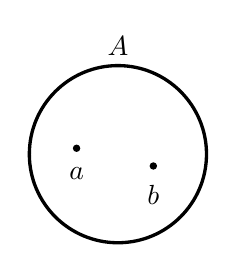
\begin{tikzpicture}[scale=.75]
		\draw[color=black, very thick](0,0) circle (1.5); 
		\node[above] at (0,1.5) {$A$};
		\filldraw (-.7,.1) circle (1.5pt) node[label=below:$a$] 
		{};
		\filldraw (.6,-.2) circle (1.5pt) node[label=below:$b$] 
		{};
	\end{tikzpicture}
	\caption{A set $A$ which contains elements $a$ and 
	$b$.}\label{set}
\end{marginfigure}

Sets are commonly visualized as circles or ovals, as in 
Figure \ref{set}, which depicts a set $A$ containing 
elements $a$ and $b$.

It is common to ``equip'' a set with a structure. For 
example, one could equip a set with a topology, as discussed in 
Section \ref{top space}.

%%%%%%%%%%%%%%%%%%%%%%%%%%%%%%%%%%%%%%%%%%%%%%%%%%%%%%%%%%%%%%%%%%

\newpage

\subsection{Comparing Different Sets}\label{compare sets}

\begin{itemize}
	\item $A$ is a \df{subset}\index{set!subset} of $B$ if every 
	element of $A$ is also an element of $B$, and we write $A 
	\subseteq B$. $A$ is a \df{proper subset} of $B$ if $A$ 
	is a subset of $B$ and $A$ is different from $B$, and we 
	write $A \subsetneq B$. See Figure \ref{subset}.
	
\begin{marginfigure}
	\centering
	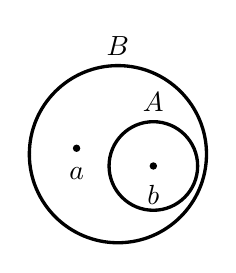
\begin{tikzpicture}[scale=.75]
		\draw[color=black, very thick](0,0) circle (1.5); 
		\node[above] at (0,1.5) {$B$};
		\filldraw (-.7,.1) circle (1.5pt) node[label=below:$a$] 
		{};
		\filldraw (.6,-.2) circle (1.5pt) node[label=below:$b$] 
		{};
		\draw[color=black, very thick](.6,-.2) circle (.75);
		\node[above] at (.6,.55) {$A$};
	\end{tikzpicture}
	\caption{The set $A = \{ b \}$ is a proper subset of the set $B 
	= \{ a,b \}$.}\label{subset}
\end{marginfigure}
	
	\item Two sets are \df{disjoint}\index{set!disjoint sets} 
	if	$A \cap B = \varnothing$.
	
	\item A set is \df{finite}\index{set!finite} if it is 
	empty or if there is a bijection
	\[
	f : A \to \{ 1, 2, \dots, n \}
	\]
	for some positive integer $n$. (See Sec \ref{func props}.) In 
	the former case, we say that $A$ has \df{cardinality} 
	0\index{set!cardinality}; in the latter case, we say that $A$ 
	has \df{cardinality} $n$. If a bijection exists between $A$ and 
	the positive integers, we say that $f$ is \df{countably 
	infinite}. If a set is finite or countably infinite, it is 
	\df{countable}\index{set!countable}. If there exists a 
	bijection between two sets, they have the same cardinality. We 
	denote the cardinality of $A$ by $|A|$. Intuitively, if you can 
	pair up
\end{itemize}

\begin{remark}
	ZXclkJZXlckLxcj...
\end{remark}

%%%%%%%%%%%%%%%%%%%%%%%%%%%%%%%%%%%%%%%%%%%%%%%%%%%%%%%%%%%%%%%%%%

\newpage

\subsection{How to Form New Sets From Given Ones}

\begin{itemize}
	\item Given some sets, we could consider the set to which 
	each of these sets is an element. We refer to this new set as 
	a \df{collection} of sets.
	
	\item Given a collection $\mc{A}$ of sets, the 
	\df{union}\index{set!union of} of the elements of 
	$\mc{A}$ is the set
	\[
	\bigcup_{A \in \mc{A}} A = \{ x \mid x \in A \text{ for 
		at least one } A \in \mc{A} \}\,.
	\]

	\item Given a collection $\mc{A}$ of sets, the 
	\df{intersection}\index{set!intersection of} of the 
	elements of $\mc{A}$ is the set
	\[
	\bigcap_{A \in \mc{A}} A = \{ x \mid x \in A \text{ for 
		every } A \in \mc{A} \}\,.
	\]

\begin{marginfigure}
	\begin{subfigure}{2in}
		\centering
		\begin{venndiagram3sets}[
			tikzoptions={scale=.5,thick},
			shade=pink
		]
			\fillA	\fillB 	\fillC
		\end{venndiagram3sets}
		\caption{Here $\mc{A} = {A, B, C}$ and the shaded region 
			illustrates $\bigcup_{X \in \mc{A}} X$ (or $A \cup B 
			\cup C$).}
	\end{subfigure}
	\begin{subfigure}{2in}
		\centering
		\begin{venndiagram3sets}[
			tikzoptions={scale=.5,thick},
			shade=pink
		]
			\fillACapBCapC
		\end{venndiagram3sets}
		\caption{Here $\mc{A} = {A, B, C}$ and the shaded region 
			illustrates $\bigcap_{X \in \mc{A}} X$ (or $A \cap B 
			\cap C$).}
	\end{subfigure}
	\begin{subfigure}{2in}
		\centering
		\begin{venndiagram2sets}[
			tikzoptions={scale=.5,thick},
			shade=pink
		]
			\fillOnlyA
		\end{venndiagram2sets}
		\caption{The shaded region illustrates $A \setminus B$.}
	\end{subfigure}
	\caption{Visualization of common set operations.}
\end{marginfigure}
	
	\item Given two sets $A$ and $B$, the 
	\df{difference}\index{set!difference of} of $A$ and $B$ is 
	the set
	\[
		A \setminus B = \{ x \mid x \in A \text{ and } x \notin B 
		\}\,.
	\]
	
	\item Let $\{ A_\alpha \}_{\alpha \in J}$ be an indexed family 
	of sets. Let $X = \bigcup_{\alpha \in J} A_\alpha$. We define 
	the \df{cartesian product}\index{set!cartesian product} of this 
	indexed family, denoted by 
	\[
		\prod_{\alpha \in J} A_\alpha\,,
	\]
	to be the set of all $J$-tuples $(x_\alpha)_{\alpha \in J}$ of 
	elements of $X$ such that $x_\alpha \in A_\alpha$ for each 
	$\alpha \in J$.
	
	\item We can also break sets down into constituent parts. The 
	\df{partition}\index{set!partition of} of a set $A$ is a 
	collection 
	of disjoint nonempty subsets of $A$ whose union is all of $A$.
\end{itemize}

\begin{marginfigure}[.25in]
	\begin{subfigure}{2in}
		\centering
		\begin{venndiagram3sets}[
			tikzoptions={scale=.5,thick},
			shade=pink
			]
			\fillACapB 	\fillACapC
		\end{venndiagram3sets}
		\caption{Visualization of the first distributive law.}
	\end{subfigure}
	\begin{subfigure}{2in}
		\centering
		\begin{venndiagram3sets}[
			tikzoptions={scale=.5,thick},
			shade=pink
			]
			\fillOnlyA
		\end{venndiagram3sets}
		\caption{Visualization of the first of DeMorgan's laws.}
	\end{subfigure}
\end{marginfigure}

\begin{theorem}[Laws of Combining Sets]
	$ $
	\begin{itemize}
		\item Set-Theoretic Distributive Laws:
		\begin{align}
			A \cap (B \cup C) &= (A \cap B) \cup (A \cap C)\,; \\
			A \cup (B \cap C) &= (A \cup B) \cap (A \cup C)\,.
		\end{align}
	
		\item DeMorgan's Laws:
		\begin{align}
			A \setminus (B \cup C)
				&= (A \setminus B) \cap (A \setminus C)\,; \\
			A \setminus (B \cap C)
				&= (A \setminus B) \cup (A \setminus C)\,.
		\end{align}
	\end{itemize}
\end{theorem}

%%%%%%%%%%%%%%%%%%%%%%%%%%%%%%%%%%%%%%%%%%%%%%%%%%%%%%%%%%%%%%%%%%
%%%%%%%%%%%%%%%%%%%%%%%%%%%%%%%%%%%%%%%%%%%%%%%%%%%%%%%%%%%%%%%%%%

\newpage

\section{Functions}

\subsection{Definition and Examples}

\begin{definition}
	$ $
	\begin{itemize}
		\item A \df{rule of assignment}\index{function!rule of 
		assignment} 
		is a subset $r$ of the cartesian product $C \times D$ of 
		two sets such that
		\[
			[(c,d) \in r \text{ and } (c,d') \in r] \Ra [d=d']\,.
		\]
		The \df{domain}\index{function!domain} and \df{image 
		set}\index{function!image set} of $r$ are defined as
		\begin{align}
			\domain r &= \{ c \mid \text{there exists } d \in D
				\text{ such that } (c,d) \in r \}\,, \\
			\image r &= \{ d \mid \text{there exists } c \in C 
			\text{ such that } (c,d) \in r \}\,.
		\end{align}
		
		\item A \df{function}\index{function} $f$ is a rule of 
		assignment $r$, together with a set $B$ that contains the 
		image set of $r$. The domain $A$ of the rule $r$ is also 
		called the \df{domain} of the function $f$; the image set 
		of $r$ is also called the \df{image set} of $f$; and the 
		set $B$ is called the 
		\df{codomain}\index{function!codomain} of $f$. We 
		write $f : A \to B$ and say ``$f$ is a function from $A$ 
		to $B$''
		
		\item If $f: A \to B$ and if $a$ is an element of $A$, we 
		denote by $f(a)$ the unique element of $B$ such that $(a, 
		f(a)) \in r$; it is called the 
		\df{value}\index{function!value of element} of $f$ at 
		$a$, or the 
		\df{image}\index{function!image of element} of $a$ 
		under $f$. We also write $a \mapsto b$.
		
		\item Let $f : A \to B$. If $A_0$ is a subset of $A$, we 
		denote by $f(A_0)$ the set $f(A_0) = \{ b \mid b = f(a) 
		\text{ for at least one } a \in A_0 \}$. This set is 
		called the \df{image}\index{function!image of subset} 
		of $A_0$ under $f$. 
		
		\item If $B_0$ is a subset of $B$, we denote by 
		$f^{-1}(B_0)$ the set $f^{-1}(B_0) = \{ a \mid f(a) \in B_0 
		\}.$ This set is called the 
		\df{preimage}\index{function!preimage} of $B_0$ under $f$. The preimage of a single-element set, say $\{ b \}$, under $f$ is called the \df{fiber}\index{function!fiber} of $f$ over $b$.
	\end{itemize}
\end{definition}

\begin{marginfigure}
	\centering
	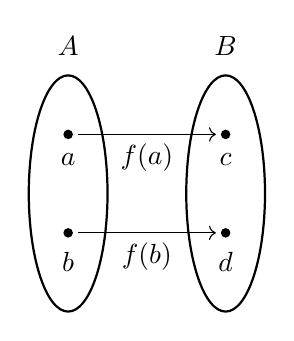
\begin{tikzpicture}
	\draw[thick] (0,0) ellipse (.5 and 1.5);
	\node[label=$A$] at (0,1.5) (A) {};
	\filldraw (0,.75) circle (1.5pt) node[label=below:$a$] (a) {};
	\filldraw (0,-.5) circle (1.5pt) node[label=below:$b$] (b) {};
	
	\draw[thick] (2,0) ellipse (.5 and 1.5);
	\node[label=$B$] at (2,1.5) (B) {};
	\filldraw (2,.75) circle (1.5pt) node[label=below:$c$] (c) {};
	\filldraw (2,-.5) circle (1.5pt) node[label=below:$d$] (d) {};
	
	\draw[->] (a) -- (c) node[midway,below] {$f(a)$};
	\draw[->] (b) -- (d) node[midway,below] {$f(b)$};
	\end{tikzpicture}
	\caption{A function $f$ between the sets $A$ and 
		$B$.}\label{function}
\end{marginfigure}

Intuitively, a function is a mapping from one set to another. 
Functions are commonly visualized as arrows between the elements 
of sets, as in Figure \ref{function}.

%%%%%%%%%%%%%%%%%%%%%%%%%%%%%%%%%%%%%%%%%%%%%%%%%%%%%%%%%%%%%%%%%%

\subsection{How to Form New Functions From Given Ones}

\begin{itemize}
	\item If $f : A \to B$ and if $A_0$ is a subset of $A$, 
	we define the \df{restriction}\index{function!restriction of} 
	of $f$ to $A_0$ to be the function mapping $A_0$ into $B$ 
	whose rule is $\{ (a,f(a)) \mid a \in A_0 \}$. It is denoted 
	by $f|A_0$, and we say ``$f$ restricted to $A_0$.''
	
	\item Given functions $f : A \to B$ and $g : B \to C$, we 
	can define the \df{composite}\index{function!composite} $g 
	\circ 
	f$ (read ``$g$ after $f$'') of $f$ and $g$ as the 
	function 
	$g \circ f : A \to C$ to be the function whose rule is
	\[
	\{ (a,c) \mid \text{For some } b \in B, f(a) = b \text{ 
		and } g(b) = c \}\,.
	\]
	
	\item If $f : A \to B$, then $f$ has a \df{left inverse}\index{function!left inverse} if there is a function $g : B \to A$ such that $g \circ f : A \to A$ is the identity map on $A$, i.e., $(g \circ f)(a) = a$, for all $a \in A$. $f$ has a \df{right inverse}\index{function!left inverse} if there is a function $h : B \to A$ such that $f \circ h : B \to B$ is the identity map on $B$.
	
	\item If $f$ is bijective, there exists a function 
	$f^{-1}$ called the \df{inverse}\index{function!inverse} of 
	$f$ 
	defined by letting $f^{-1}(b)$ be the unique $a$ such 
	that $f(a) = b$.
\end{itemize}

%%%%%%%%%%%%%%%%%%%%%%%%%%%%%%%%%%%%%%%%%%%%%%%%%%%%%%%%%%%%%%%%%%

\subsection{Properties a Function Can Have}\label{func props}
\begin{itemize}
	\item A function $f : A \to B$ is 
	\df{injective}\index{function!injective} (or 
	\df{one-to-one}\index{function!one-to-one}) if
	\[
		[f(a) = f(a')] \Ra [a = a']\,,
	\]
	and \df{surjective}\index{function!surjective} (or 
	\df{onto}\index{function!onto}) if 
	\[
		[b \in B] \Ra [b = f(a) \text{ for at least one } a 
		\in A]\,.
	\]
	If $f$ is both injective and surjective, it is said to be 
	\df{bijective}\index{function!bijective} (or is called a 
	\df{one-to-one correspondence}\index{function!one-to-one 
	correspondence}).
\end{itemize}

\begin{marginfigure}
\begin{subfigure}{2in}
	\centering
	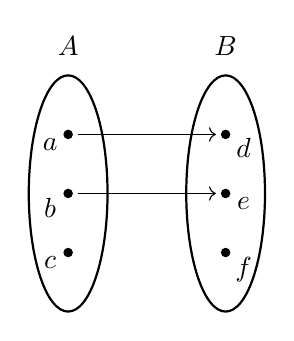
\begin{tikzpicture}
	\draw[thick] (0,0) ellipse (.5 and 1.5);
	\node[label=$A$] at (0,1.5) (A) {};
	\filldraw (0,.75) circle (1.5pt) 
	node[label={[xshift=-6.5pt,yshift=5.5pt]below:$a$}] (a) {};
	\filldraw (0,0) circle (1.5pt) 
	node[label={[xshift=-6.5pt,yshift=5.5pt]below:$b$}] (b) {};;
	\filldraw (0,-.75) circle (1.5pt) 
	node[label={[xshift=-6.5pt,yshift=5.5pt]below:$c$}] (c) {};
	
	\draw[thick] (2,0) ellipse (.5 and 1.5);
	\node[label=$B$] at (2,1.5) (B) {};
	\filldraw (2,.75) circle (1.5pt) 
	node[label={[xshift=6.5pt,yshift=5.5pt]below:$d$}] (d) {};
	\filldraw (2,0) circle (1.5pt) 
	node[label={[xshift=6.5pt,yshift=5.5pt]below:$e$}] (e) {};
	\filldraw (2,-.75) circle (1.5pt) 
	node[label={[xshift=6.5pt,yshift=5.5pt]below:$f$}] (f) {};
	
	\draw[->] (a) -- (d);
	\draw[->] (b) -- (e);
	\end{tikzpicture}
	\caption{This function is injective but not 
	surjective.}\label{inj function}
\end{subfigure}
\begin{subfigure}{2in}
	\centering
	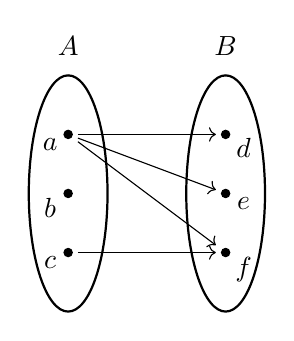
\begin{tikzpicture}
	\draw[thick] (0,0) ellipse (.5 and 1.5);
	\node[label=$A$] at (0,1.5) (A) {};
	\filldraw (0,.75) circle (1.5pt) 
	node[label={[xshift=-6.5pt,yshift=5.5pt]below:$a$}] (a) {};
	\filldraw (0,0) circle (1.5pt) 
	node[label={[xshift=-6.5pt,yshift=5.5pt]below:$b$}] (b) {};;
	\filldraw (0,-.75) circle (1.5pt) 
	node[label={[xshift=-6.5pt,yshift=5.5pt]below:$c$}] (c) {};
	
	\draw[thick] (2,0) ellipse (.5 and 1.5);
	\node[label=$B$] at (2,1.5) (B) {};
	\filldraw (2,.75) circle (1.5pt) 
	node[label={[xshift=6.5pt,yshift=5.5pt]below:$d$}] (d) {};
	\filldraw (2,0) circle (1.5pt) 
	node[label={[xshift=6.5pt,yshift=5.5pt]below:$e$}] (e) {};
	\filldraw (2,-.75) circle (1.5pt) 
	node[label={[xshift=6.5pt,yshift=5.5pt]below:$f$}] (f) {};
	
	\draw[->] (a) -- (d);
	\draw[->] (a) -- (e);
	\draw[->] (a) -- (f);
	\draw[->] (c) -- (f);
	\end{tikzpicture}
	\caption{This function is surjective but not 
	injective.}\label{surj function}
\end{subfigure}
\begin{subfigure}{2in}
	\centering
	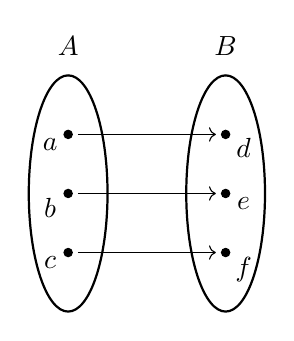
\begin{tikzpicture}
	\draw[thick] (0,0) ellipse (.5 and 1.5);
	\node[label=$A$] at (0,1.5) (A) {};
	\filldraw (0,.75) circle (1.5pt) 
	node[label={[xshift=-6.5pt,yshift=5.5pt]below:$a$}] (a) {};
	\filldraw (0,0) circle (1.5pt) 
	node[label={[xshift=-6.5pt,yshift=5.5pt]below:$b$}] (b) {};;
	\filldraw (0,-.75) circle (1.5pt) 
	node[label={[xshift=-6.5pt,yshift=5.5pt]below:$c$}] (c) {};
	
	\draw[thick] (2,0) ellipse (.5 and 1.5);
	\node[label=$B$] at (2,1.5) (B) {};
	\filldraw (2,.75) circle (1.5pt) 
	node[label={[xshift=6.5pt,yshift=5.5pt]below:$d$}] (d) {};
	\filldraw (2,0) circle (1.5pt) 
	node[label={[xshift=6.5pt,yshift=5.5pt]below:$e$}] (e) {};
	\filldraw (2,-.75) circle (1.5pt) 
	node[label={[xshift=6.5pt,yshift=5.5pt]below:$f$}] (f) {};
	
	\draw[->] (a) -- (d);
	\draw[->] (b) -- (e);
	\draw[->] (c) -- (f);
	\end{tikzpicture}
	\caption{This function is bijective.}\label{bij function}
\end{subfigure}
\caption{Visualizations of injective, surjective, and bijective 
functions.}\label{function examples}
\end{marginfigure}

The basic idea is that if we can find a bijective function 
between two sets, then they are the same ``size'' or 
``cardinality.'' (See Section \ref{compare sets}.)
These properties are illustrated in Figure \ref{function 
examples}. 

The following lemma comes in handy for showing that a given 
function is bijective

\begin{lemma}
	Let $f : A \to B$. If there are functions $g : B \to A$ and 
	$h : B \to A$ such that $g(f(a)) = a$ for every $a$ in $A$ 
	and $f(h(b)) = b$ for every $b$ in $B$, then $f$ is bijective 
	and $g = h = f^{-1}$.
\end{lemma}

\begin{example}
	A \df{permutation}\index{function!permutation} of a set $A$ is simply a bijection from $A$ to itself.
\end{example}

%%%%%%%%%%%%%%%%%%%%%%%%%%%%%%%%%%%%%%%%%%%%%%%%%%%%%%%%%%%%%%%%%%
%%%%%%%%%%%%%%%%%%%%%%%%%%%%%%%%%%%%%%%%%%%%%%%%%%%%%%%%%%%%%%%%%%

\newpage

\section{Relations}

\subsection{Definition and Examples}

\begin{definition}[Relation]
	A \df{binary relation}\index{binary relation} on a set $A$ is a subset $C$ of the cartesian product $A \times A$. We use the notation $xCy$ to mean the same thing as $(x,y) \in C$, and we say ``$x$ is in the relation $C$ to $y$.''
\end{definition}

Remark: This is weaker than a rule of assignment in the sense 
that a given element is allowed to be assigned to more than one 
value of the second set. A function $f:A \to A$ is a special case 
of a relation. Note that both sets are always the same 
in the case of a relation.

For a given relation $C$ on the set $A$, 
\begin{itemize}
	\item A relation is \df{reflexive}\index{binary relation!reflexive} 
	if $xCx$ for every $x$ in $A$.
	
	\item A relation is \df{symmetric}\index{binary relation!symmetric} 
	if $xCy$ implies $yCx$.
	
	\item A relation is 
	\df{transitive}\index{binary relation!transitive} if $xCy$ and $yCz$ 
	together implies $xCz$.
	
	\item A relation is 
	\df{comparable}\index{binary relation!comparable} if for every $x$ 
	and $y$ in $A$ for which $x \neq y$, either $xCy$ or $yCx$.
	
	\item A relation is 
	\df{nonreflexive}\index{binary relation!nonreflexive} if for no $x$ 
	in $A$ does the relation $xCx$ hold.
\end{itemize}

%%%%%%%%%%%%%%%%%%%%%%%%%%%%%%%%%%%%%%%%%%%%%%%%%%%%%%%%%%%%%%%%%%

\subsection{Equivalence Relations}\label{eq 
relation properties}

\begin{definition}[Equivalence Relation]
	An \df{equivalence relation}\index{binary relation!equivalence 
	relation} on a 
	set $A$ is a relation $C$ on $A$ which is reflexive, 
	symmetric, and transitive. We often use $\sim$ for an 
	equivalence relation instead of $C$.
\end{definition}

\begin{itemize}
	\item Given an equivalence relation $\sim$ on a set $A$ and 
	an element $x$ of $A$, we define the \df{equivalence 
	class}\index{binary relation!equivalence class} determined by $x$ as
	\[
		\{ y \mid y \sim x \}\,.
	\]
	If $C$ is an equivalence class, any element of $C$ is called a \df{representative}\index{binary relation!representative of an equivalence class} of the class $C$.
	Two equivalent classes are either disjoint or equal, and the 
	collection of equivalence classes of a set $A$ partition $A$.
\end{itemize}

%%%%%%%%%%%%%%%%%%%%%%%%%%%%%%%%%%%%%%%%%%%%%%%%%%%%%%%%%%%%%%%%%%

\subsection{Order Relations}

\begin{definition}[Order Relation]
	An \df{order relation}\index{binary relation!order relation} on a 
	set $A$ is a relation $C$ on $A$ which is comparable, 
	nonreflexive, and transitive. We often use $<$ for an 
	order relation instead of $C$.
\end{definition}

Suppose that $A$ and $B$ are two sets with order 
relations. We say that $A$ and $B$ have the same \df{order 
type}\index{binary relation!order type} if there is a bijective 
correspondence 
between them that preserves order.

\begin{example}
	Suppose that $A$ and $B$ are two sets with order relations 
	$<_A$ and $<_B$ respectively. Define an order relation $<$ on 
	$A \times B$ by defining
	\[
		a_1 \times b_1 < a_2 \times b_2
	\]
	if $a_1 <_A a_2$ or if $a_1 = a_2$ and $b_1 <_B b_2$. This is 
	called the \df{dictionary order 
	relation}\index{binary relation!dictionary order relation}.
\end{example}

%%%%%%%%%%%%%%%%%%%%%%%%%%%%%%%%%%%%%%%%%%%%%%%%%%%%%%%%%%%%%%%%%%
%%%%%%%%%%%%%%%%%%%%%%%%%%%%%%%%%%%%%%%%%%%%%%%%%%%%%%%%%%%%%%%%%%

\newpage

\section{Least Upper Bound Property}

\begin{definition}
	$ $
	\begin{itemize}
		\item Suppose that $A$ is a set ordered by the relation 
		$<$. Let $A_0$ be a subset of $A$. We say the element of 
		$b$ is the \df{largest element}\index{set!largest element 
		of} of 
		$A_0$ if $b \in A_0$ and if $x \leq b$ for every $x \in 
		A_0$. Similarly, we say that $a$ is the \df{smallest 
		element}\index{set!smallest element of} of $A_0$ if $a 
		\in A_0$ 
		and if $a \leq x$ for every $x \in A_0$.
		
		\item We say that the subset $A_0$ of $A$ is \df{bounded 
		above}\index{set!bounded above} if there is an element 
		$b$ of $A$ such that $x \leq b$ for every $x \in A_0$; 
		the element $b$ is called an \df{upper 
		bound}\index{set!upper 
		bound} for $A_0$. If the set of all upper bounds for 
		$A_0$ has a smallest element, that element is called the 
		\df{least upper bound}\index{set!least upper bound}, or 
		the 
		\df{supremum}\index{set!supremum}, of $A_0$. It is 
		denoted by 
		$\sup A_0$.
		
		\item Similarly, $A_0$ is \df{bounded 
		below}\index{set!bounded below} if there is an element 
		$a$ of $A$ such that $a \leq x$ for every $x \in A_0$; 
		the element $a$ is called a \df{lower 
		bound}\index{set!lower 
		bound} for $A_0$. If the set of all lower bounds for 
		$A_0$ has a largest element, that element is called the 
		\df{greatest lower bound}\index{set!greatest lower 
		bound}, or 
		the \df{infimum}\index{set!infimum}, of $A_0$. It is 
		denoted 
		by $\inf A_0$.
		
		\item An ordered set $A$ is said to have the \df{least 
		upper bound property}\index{set!least upper bound 
		property} 
		if every nonempty subset $A_0$ of $A$ that is bounded 
		above has a least upper bound.
	\end{itemize}
\end{definition}

The real numbers have the least upper bound property.

%%%%%%%%%%%%%%%%%%%%%%%%%%%%%%%%%%%%%%%%%%%%%%%%%%%%%%%%%%%%%%%%%%
%%%%%%%%%%%%%%%%%%%%%%%%%%%%%%%%%%%%%%%%%%%%%%%%%%%%%%%%%%%%%%%%%%



























\chapter{Logic}

Logic provides the materials needed for a rigorous theory of how 
to prove theorems and build axiomatic systems such as axiomatic 
set theory. It contains fascinating theorems with widespread 
implications such as G\"odel's infamous Incompleteness Theorems. 
The information in this chapter is based on Shoenfield's classic 
\emph{Mathematical Logic} (1967).

%%%%%%%%%%%%%%%%%%%%%%%%%%%%%%%%%%%%%%%%%%%%%%%%%%%%%%%%%%%%%%%%%%

\newpage

\section{Notation}

\begin{itemize}
	\item \bt{u} and \bt{v} are syntactical variables which vary 
	through all expressions.
	
	\item \bt{A}, \bt{B}, \bt{C}, and \bt{D} are syntactical 
	variables which vary through formulas.
	
	\item \bt{x}, \bt{y}, \bt{z}, and \bt{w} are syntactical 
	variables which vary through variables.
	
	\item \bt{f} and \bt{g} are syntactical variables which vary 
	through function symbols.
	
	\item \bt{p} and \bt{q} are syntactical variables which vary 
	through predicate symbols.
	
	\item \bt{e} is a syntactical variables which varies through 
	constants.
	
	\item \bt{a}, \bt{b}, \bt{c}, and \bt{d} are syntactical  
	variables which vary through terms.
	
	\item $\bt{b}_{\nbts{x}}[\nbts{a}]$ 
	designates the expression obtained from \bt{b} by replacing 
	all occurrences of $\nbts{x}$ by $\nbts{a}$ respectively.
	
	\item $\bt{A}_{\nbts{x}}[\nbts{a}]$ 
	designates the expression obtained from \bt{A} by replacing 
	all free occurrences of $\nbts{x}$ by $\nbts{a}$ respectively.
	
	\item \bt{i} and \bt{j} are syntactical variables which vary 
	through names.
\end{itemize}

%%%%%%%%%%%%%%%%%%%%%%%%%%%%%%%%%%%%%%%%%%%%%%%%%%%%%%%%%%%%%%%%%%

\newpage

\section{Functions and Predicates}

Main Idea: Functions assign a collection of elements from one set 
to a single element of another set. Predicates represent some 
relationship between a collection of elements from a set.

\begin{definition}[$n$-tuple]
	An \df{$n$-tuple}\index{logic!$n$-tuple} in $A$ is a sequence 
	of $n$ (not necessarily	distinct) objects in $A$.
\end{definition}

We write $(a_1, a_2, \cdots, a_n)$ for the $n$-tuple consisting of 
the objects $a_1, a_2, \cdots, a_n$ in that order. We agree that 
there is exactly one 0-tuple in $A$, and we designate it by ( ).

\begin{definition}[Functions]
	A mapping from the set of $n$-tuples in $A$ to $B$ is called an 
	\df{$n$-ary function from $A$ to $B$}\index{logic!function}.
\end{definition}

\begin{example}[Truth Functions]
	A \df{truth function}\index{logic!truth function} is a function 
	from the set of truth values, $\{ \bt{T}, \bt{F} \}$, to the 
	set of truth values. We have
	\begin{itemize}
		\item the \df{and} truth function:
		\begin{align*}
			H_\land(\bt{T},\bt{T}) &= \bt{T}\,, \\
			H_\land(\bt{T},\bt{F}) &= H_\land(\bt{F},\bt{T})
				= H_\land(\bt{F},\bt{F}) = \bt{F}\,.
		\end{align*}
		\item the \df{or} truth function:
		\begin{align*}
			H_\lor(\bt{T},\bt{T}) &= H_\lor(\bt{T},\bt{F})
				= H_\lor(\bt{F},\bt{T}) = \bt{T}\,, \\
			H_\lor(\bt{F},\bt{F}) &= \bt{F}\,.
		\end{align*}
		\item the \df{if ... then} truth function:
		\begin{align*}
			H_\to(\bt{T},\bt{T}) &= H_\to(\bt{F},\bt{T})
				= H_\to(\bt{F},\bt{F}) = \bt{T}\,, \\
			H_\to(\bt{T},\bt{F}) &= \bt{F}\,.
		\end{align*}
		\item the \df{if and only if} truth function:
		\begin{align*}
			H_\lra(\bt{T},\bt{T}) &= H_\lra(\bt{F},\bt{F})
				= \bt{T}\,, \\
			H_\lra(\bt{T},\bt{F}) &= H_\lra(\bt{F},\bt{T})
				= \bt{F}\,.
		\end{align*}
		\item the \df{not} truth function:
		\[
			H_\neg(\bt{T}) = \bt{F}\,,
			\quad 
			H_\neg(\bt{F}) = \bt{T}\,.
		\]
	\end{itemize}
\end{example}

\begin{definition}[Predicate]
	A subset of the set of $n$-tuples in $A$ is called an 
	\df{$n$-ary predicate in $A$}\index{logic!predicate}.
\end{definition}

If $P$ represents such a predicate, then $P(a_1, \cdots, a_n)$ 
means that the $n$-tuple $(a_1, \cdots, a_n)$ is in $P$. We say 
\df{unary} for 1-ary and \df{binary} for 2-ary. Note that a unary 
function from $A$ to $B$ is a mapping from $A$ to $B$, and that a 
unary predicate in $A$ is a subset of $A$.

%%%%%%%%%%%%%%%%%%%%%%%%%%%%%%%%%%%%%%%%%%%%%%%%%%%%%%%%%%%%%%%%%%
%%%%%%%%%%%%%%%%%%%%%%%%%%%%%%%%%%%%%%%%%%%%%%%%%%%%%%%%%%%%%%%%%%

\newpage

\section{First-Order Languages}

Main Idea: First-order languages belong to the syntactical study of 
axiom systems. They describe the symbols to be used.

\begin{definition}[First-order Language]
	A \df{first-order language}\index{logic!first-order language} 
	has as symbols the following:
	\begin{enumerate}
		\item[a)] the variables
		\[ x,y,z,w,x',y',z',w',x'', \dots \,; \]
		
		\item[b)] for each $n$, the $n$-ary function symbols and 
		the $n$-ary predicate symbols;
		
		\item[c)] the symbols $\neg$, $\lor$, and $\exists$.
	\end{enumerate}
\end{definition}

Remark: The equality symbol = must be among the binary predicate 
symbols.

The first-order language $L'$ is an 
\df{extension}\index{logic!extension of language} of the 
first-order language $L$ if every nonlogical symbol of $L$ is a 
nonlogical symbol of $L'$.

\begin{definition}[Designators]
	$ $
	\begin{itemize}
		\item We define the \df{terms}\index{logic!terms} of a 
		first-order language by the generalized inductive 
		definition:
		\begin{enumerate}
			\item[i)] a variable is a term;
				
			\item[ii)] if $\bt{u}_1, \cdots, \bt{u}_n$ are 
			terms and \bt{f} is $n$-ary, then 
			$\bt{f}\bt{u}_1 \cdots \bt{u}_n$ is a term.
		\end{enumerate}
		
		\item An \df{atomic formula}\index{logic!atomic formula} is 
		an expression of the form $\bt{p}\bt{a}_1 \cdots \bt{a}_n$ 
		where \bt{p} is $n$-ary. We define the 
		\df{formulas}\index{logic!formulas} of a first-order 
		language by the generalized inductive definition:
		\begin{enumerate}
			\item[i)] an atomic formula is a formula;
			
			\item[ii)] if \bt{u} is a formula, then $\neg \bt{u}$ 
			is a formula;
			
			\item[iii)] if \bt{u} and \bt{v} are formulas, then 
			$\lor \bt{u}\bt{v}$ is a formula;
			
			\item[iv)] if \bt{u} is a formula, then $\exists \bt{x} 
			\bt{u}$ is a formula.
		\end{enumerate}
		\item A \df{designator}\index{logic!designator} is an 
		expression which is either a term or a formula.
	\end{itemize}
\end{definition}

%%%%%%%%%%%%%%%%%%%%%%%%%%%%%%%%%%%%%%%%%%%%%%%%%%%%%%%%%%%%%%%%%%
%%%%%%%%%%%%%%%%%%%%%%%%%%%%%%%%%%%%%%%%%%%%%%%%%%%%%%%%%%%%%%%%%%

\newpage

\section{Structures}

Main Idea: Structures describe the semantics, the meaning, of 
first-order languages; We attach meanings to the symbols. 
Individuals of the structure are given names. Add names to $L$ to 
get $L(\ms{A})$. Assign every variable-free term of $L(\ms{A})$ to 
an individual of the structure. Closed formulas of $L(\ms{A})$ are 
then given truth values, specifying if they're true in the 
structure. Then can say \bt{A} is valid in $\ms{A}$ if every 
instantiation of \bt{A} is true in $\ms{A}$. A model is a structure 
for a theory of a language in which all the nonlogical axioms of 
the theory are valid.

%%%%%%%%%%%%%%%%%%%%%%%%%%%%%%%%%%%%%%%%%%%%%%%%%%%%%%%%%%%%%%%%%%

\subsection{Definition}

\begin{definition}[Structure]
	Let $L$ be a first-order language. A 
	\df{structure}\index{logic!structure} $\ms{A}$ for $L$ consists 
	of the following things:
	\begin{enumerate}
		\item[i)] A nonempty set $| \ms{A} |$, called the 
		\df{universe} of $\ms{A}$. The elements of $| \ms{A} |$ are 
		called the \df{individuals} of $\ms{A}$.
		
		\item[ii)] For each $n$-ary function symbol \bt{f} of $L$, 
		an $n$-ary function $\bt{f}_\ms{A}$ from $| \ms{A} |$ to $| 
		\ms{A} |$.
		
		\item[iii)] For each $n$-ary predicate symbol \bt{p} of $L$ 
		other than =, an $n$-ary predicate $\bt{p}_\ms{A}$ in $| 
		\ms{A} |$.
	\end{enumerate}
\end{definition}

For each individual $a$ of $\ms{A}$, we choose a new constant, 
called the \df{name}\index{logic!name} of $a$. The first-order 
language obtained from $L$ by adding all the names of individuals 
of $\ms{A}$ is designated by $L(\ms{A})$. A formula \bt{A} is 
\df{closed}\index{logic!closed formula} if no variable is free in 
\bt{A}.

%%%%%%%%%%%%%%%%%%%%%%%%%%%%%%%%%%%%%%%%%%%%%%%%%%%%%%%%%%%%%%%%%%

\subsection{Individuals and Truth of Formulas in $\ms{A}$}

For each variable-free term \bt{a} of $L(\ms{A})$:
\begin{itemize}
	\item If \bt{a} is a name, $\ms{A}(\bt{a})$ is the individual 
	of which \bt{a} is the name.
	
	\item If \bt{a} is $\bt{f}\bt{a}_1 \cdots \bt{a}_n$, 
	$\ms{A}(\bt{a})$ is $\bt{f}_\ms{A} \left( \ms{A}(\bt{a}_1), 
	\cdots, \ms{A}(\bt{a}_n) \right)$.
\end{itemize}

\noindent
For each closed formula \bt{A} of $L(\ms{A})$:
\begin{itemize}
	\item If \bt{A} is $\bt{a} = \bt{b}$, $\ms{A}(\bt{A}) = \bt{T}$ 
	if and only if $\ms{A}(\bt{a}) = \ms{A}(\bt{b})$.
	
	\item If \bt{A} is $\bt{p}\bt{a}_1 \cdots \bt{a}_n$, where 
	\bt{p} is not =, $\ms{A}(\bt{A}) = \bt{T}$ if and only if 
	$\bt{p}_\ms{A} \left( \ms{A}(\bt{a}_1), \cdots, 
	\ms{A}(\bt{a}_n) \right)$.
	
	\item If \bt{A} is $\neg \bt{B}$, $\ms{A}(\bt{A})$ is 
	$\Hneg{}(\ms{A}(\bt{B}))$.
	
	\item If \bt{A} is $\lor \bt{B} \bt{C}$, $\ms{A}(\bt{A})$ 
	is $\Hor{}(\ms{A}(\bt{B}),\ms{A}(\bt{C}))$.
	
	\item If \bt{A} is $\existsx{}\bt{B}$, $\ms{A}(\bt{A}) = 
	\bt{T}$ if and 
	only if $\ms{A}(\Bxi{}) = \bt{T}$ for some \bt{i} in 
	$L(\ms{A})$.
\end{itemize}

If \bt{A} is a formula of $L$, an $\ms{A}$-instance of \bt{A} is a 
closed formula of the form $\bt{A}[\bt{i}_1, \dots, \bt{i}_n]$ in 
$L(\ms{A})$.
A formula \bt{A} is \df{valid}\index{logic!valid formula} in 
$\ms{A}$ if $\ms{A}(\bt{A}') = \bt{T}$ for every $\ms{A}$-instance 
$\bt{A}'$ of \bt{A}.
A formula is \df{elementary}\index{logic!elementary formula}  if it 
is either an atomic formula or an instantiation.

%%%%%%%%%%%%%%%%%%%%%%%%%%%%%%%%%%%%%%%%%%%%%%%%%%%%%%%%%%%%%%%%%%
%%%%%%%%%%%%%%%%%%%%%%%%%%%%%%%%%%%%%%%%%%%%%%%%%%%%%%%%%%%%%%%%%%

\newpage

\section{First-Order Theories}

Main Idea: The primary object of a formal system is to provide a 
framework for proving theorems.

%%%%%%%%%%%%%%%%%%%%%%%%%%%%%%%%%%%%%%%%%%%%%%%%%%%%%%%%%%%%%%%%%%

\subsection{Definition}

\begin{definition}[Formal System]
	A \df{formal system} $F$ consists of a language $L(F)$, axioms 
	of $F$, and rules of inference of $F$ which enable us to 
	conclude theorems from the axioms.
\end{definition}

\begin{definition}[First-Order Theory]
	A \df{first-order theory}\index{logic!first-order theory}, or 
	simply a \df{theory}, is a formal system $T$ such that
	\begin{enumerate}
		\item[i)] the language of $T$ is a first-order language;
		
		\item[ii)] the axioms of $T$ are the logical axioms of 
		$L(T)$ and certain further axioms called the \df{nonlogical 
		axioms};
		
		\item[iii)] the rules of $T$ are the expansion rule, the 
		contraction rule, the associative rule, the cut rule, and 
		the $\exists$-introduction rule.
	\end{enumerate}
\end{definition}

The logical axioms\index{logic!logical axioms} are the following:
\begin{itemize}
	\item Propositional axiom: $\propax$
	
	\item Substitution axiom: $\subax$
	
	\item Identity axiom: $\idax$
	
	\item Equality axiom: 
	\[ \eqax \] or \[ \eqpredax \]
\end{itemize}

The rules are the following:
\begin{itemize}
	\item Expansion: Infer $\bt{B} \lor \bt{A}$ from \bt{A}.
	
	\item Contraction: Infer \bt{A} from $\bt{A} \lor \bt{A}$.
	
	\item Associative: Infer $(\bt{A} \lor \bt{B}) \lor \bt{C}$ 
	from $\bt{A} \lor (\bt{B} \lor \bt{C})$.
	
	\item Cut: Infer $\bt{B} \lor \bt{C}$ from $\bt{A} \lor \bt{B}$ 
	and $\neg \bt{A} \lor \bt{C}$.
	
	\item $\exists$-Introduction: If \bt{x} is not free in \bt{B}, 
	infer $\existsx \bt{A} \ra \bt{B}$ from $\bt{A} \ra \bt{B}$.
\end{itemize}

%%%%%%%%%%%%%%%%%%%%%%%%%%%%%%%%%%%%%%%%%%%%%%%%%%%%%%%%%%%%%%%%%%

\subsection{Models of Theories}

\begin{definition}[Model]
	A \df{model}\index{logic!model} of a theory $T$ is a structure 
	for $L(T)$ in which all the nonlogical axioms of $T$ are valid. 
	A formula is \df{valid in $T$} if it is valid in every model of 
	$T$; equivalently, if it is a logical consequence of the 
	nonlogical axioms of $T$.
\end{definition}

\begin{example}[Elementary Theory of Groups, $G$]
	The only nonlogical symbol of $G$ is the binary function symbol 
	$\cdot$. The nonlogical axioms of $G$ are:
	\begin{enumerate}
		\item[G1.] $(x \cdot y) \cdot z = x \cdot (y \cdot z)$\,.
		
		\item[G2.] $\exists x (\forall y(x \cdot y = y) \land 
		\forall y \exists z (z \cdot y = x))$\,.
	\end{enumerate}
	
	A model of $G$ would be the set of invertible $2 \times 2$ 
	matrices under matrix multiplication.
\end{example}

%%%%%%%%%%%%%%%%%%%%%%%%%%%%%%%%%%%%%%%%%%%%%%%%%%%%%%%%%%%%%%%%%%

\subsection{Definitions Relevant to Theories}

\begin{itemize}
	\item A theory $T'$ is an \df{extension}\index{logic!extension 
	of theory} of a theory $T$ if $L(T')$ is an extension of $L(T)$ 
	and every theorem of $T$ is a theorem of $T'$. A 
	\df{conservative extension} of $T$ is an extension $T'$ of $T$ 
	such that every formula of $T$ which is a theorem of $T'$ is 
	also a theorem of $T$. The theories	$T$ and $T'$ are 
	\df{equivalent}\index{logic!equivalent theories} if each is an 
	extension of the other, i.e., they have the same language and 
	the same theorems.
	
	\item A theory $T$ is 
	\df{inconsistent}\index{logic!inconsistent} if every formula of 
	$T$ is a theorem of $T$; otherwise $T$ is 
	\df{consistent}\index{logic!consistent}
	
	\item A formula \bt{A} of $T$ is 
	\df{undecidable}\index{logic!undecidable} in $T$ if neither 
	\bt{A} nor $\neg \bt{A}$ is a theorem of $T$; otherwise \bt{A} 
	is \df{decidable}\index{logic!decidable} in $T$.
	
	\item A theory is \df{complete}\index{logic!complete} if it is 
	consistent and if every closed formula in $T$ is decidable in 
	$T$.
	
	\item A theory is \df{open}\index{logic!open theory} if all of 
	its nonlogical axioms are open (do not contain quantifiers).
\end{itemize}

%%%%%%%%%%%%%%%%%%%%%%%%%%%%%%%%%%%%%%%%%%%%%%%%%%%%%%%%%%%%%%%%%%

\subsection{Truth of Formulas of a Theory}

\begin{definition}[Truth Valuation]
	A \df{truth valuation}\index{logic!truth valuation for a 
	theory}	for $T$ is a mapping from the set of elementary 
	formulas in $T$ to the set of truth values.
\end{definition}

We define a truth value $V(\bt{A})$ for every formula \bt{A} by 
induction:
\begin{itemize}
	\item If \bt{A} is elementary, then $V(\bt{A})$ is already 
	defined;
	
	\item If \bt{A} is $\neg \bt{B}$, then $V(\bt{A}) = 
	\Hneg{}(V(\bt{B}))$;
	
	\item If \bt{A} is $\lor \bt{B} \bt{C}$, then $V(\bt{A}) = 
	\Hor{}(V(\bt{B}),V(\bt{C}))$.
\end{itemize}

%%%%%%%%%%%%%%%%%%%%%%%%%%%%%%%%%%%%%%%%%%%%%%%%%%%%%%%%%%%%%%%%%%

\subsection{Theorems in First-Order Theories}

\begin{theorem}[Validity Theorem]
	If $T$ is a theory, then every theorem of $T$ is valid in $T$.
\end{theorem}

%%%%%%%%%%%%%%%%%%%%%%%%%%%%%%%%%%%%%%%%%%%%%%%%%%%%%%%%%%%%%%%%%%
%%%%%%%%%%%%%%%%%%%%%%%%%%%%%%%%%%%%%%%%%%%%%%%%%%%%%%%%%%%%%%%%%%

\newpage

\section{The Characterization Problem}

\begin{definition}[Characterization Problem]
	The \df{characterization problem}\index{logic!characterization 
	problem} for a formal system $F$ is the following: find a 
	necessary and sufficient condition that a formula of $F$ be a 
	theorem of $F$.
\end{definition}

Remark: We consider the characterization problem for theories.

%%%%%%%%%%%%%%%%%%%%%%%%%%%%%%%%%%%%%%%%%%%%%%%%%%%%%%%%%%%%%%%%%%

\subsection{The Reduction Theorem}

Main Idea: To solve the characterization problem for all theories, 
it suffices to solve it for theories with no nonlogical axioms.

\begin{theorem}[Reduction Theorem]
	Let $\Gamma$ be a set of formulas in the theory $T$, and let 
	$A$ be a formula of $T$. Then \bt{A} is a theorem of 
	$T[\Gamma]$ iff there is a theorem of $T$ of the form $\bt{B}_1 
	\ra \dots \ra \bt{B}_n \ra \bt{A}$, where each $\bt{B}_i$ is 
	the closure of a formula in $\Gamma$.
\end{theorem}

\begin{theorem}[Reduction Theorem for Consistency]
	Let $\Gamma$ be a nonempty set of formulas in the theory $T$. 
	Then $T[\Gamma]$ is inconsistent iff there is a theorem of $T$ 
	which is a disjunction of negations of closures of distinct 
	formulas in $\Gamma$.
\end{theorem}

\begin{corollary}
	Let $\bt{A}'$ be the closure of \bt{A}. Then \bt{A} is a 
	theorem of $Y$ iff $T[\neg \bt{A}']$ is inconsistent.
\end{corollary}

%%%%%%%%%%%%%%%%%%%%%%%%%%%%%%%%%%%%%%%%%%%%%%%%%%%%%%%%%%%%%%%%%%

\subsection{Solutions to the Characterization Problem}

A trivial solution is that a formula is a theorem if and only if it 
has a proof.

\subsubsection{The Completeness Theorem}\index{logic!completeness 
theorem}

Main Idea: The completeness theorem, in either form, establishes an 
equivalence between a syntactical concept and a semantical concept. 
That is, it deals with concrete and abstract objects.

\begin{theorem}[Completeness Theorem, First Form (G\"odel)]
	A formula \bt{A} of a theory $T$ is a theorem of $T$ iff it is 
	valid in $T$.
\end{theorem}

\begin{theorem}[Completeness Theorem, Second Form]
	A theory $T$ is consistent iff it has a model.
\end{theorem}

The second form is proved using the concept of Henkin theories and 
special constants. It is outlined below.

\begin{definition}
	A Henkin theory\index{logic!Henkin theory} is a theory such 
	that each closed instantiation $\existsx \bt{A}$ of $T$, there 
	is a constant \bt{e} such that \\ $\vdash_T \existsx \bt{A} \ra 
	\bt{A}_\bt{x}[\bt{e}]$.
\end{definition}

One can extend any consistent theory to a Henkin theory by adding a 
special constant\index{logic!special constant} $\bt{r} = c_{\existsx
\bt{A}}$ for every case where $\existsx \bt{A}$ is a theorem, yet 
there is no such \bt{e}. If \bt{r} is the special constant for 
$\existsx \bt{A}$, then the formula $\existsx \bt{A} \ra 
\bt{A}_\bt{x}[\bt{r}]$ is called the \df{special axiom for} 
\bt{r}\index{logic!special axiom}. One can then extend this theory 
to a complete Henkin theory, which one can prove has a model. After 
showing that a theory has a model if its extension has a model, one 
can conclude that the original theory has a model.

%%%%%%%%%%%%%%%%%%%%%%%%%%%%%%%%%%%%%%%%%%%%%%%%%%%%%%%%%%%%%%%%%%

\subsubsection{The Consistency Theorem}

Main Idea: The consistency theorem deals only with concrete objects 
and is therefore finitary. Say we have a 
model of an open theory. The completeness theorem gives a proof of 
the consistency of the theory. The consistency theorem then allows 
us to convert this into a finitary proof of the consistency of the 
theory.

We start with some necessary definitions.

\begin{itemize}
	\item A theory is \df{open}\index{logic!open theory} if all of 
	its nonlogical axioms are open (do not contain quantifiers).
	
	\item A formula is a 
	\df{quasi-tautology}\index{logic!quasi-tautolgy} if it is a 
	tautological consequence of instances of identity axioms and 
	equality axioms.
\end{itemize}

\begin{theorem}[The Consistency Theorem (Hilbert-Ackermann)]
	An open theory $T$ is inconsistent if and only if there is a 
	quasi-tautology which is a disjunction of negations of 
	instances of nonlogical axioms of $T$.
\end{theorem}

%%%%%%%%%%%%%%%%%%%%%%%%%%%%%%%%%%%%%%%%%%%%%%%%%%%%%%%%%%%%%%%%%%

\subsubsection{Herbrand's Theorem}

Main Idea: Herbrand's theorem is a finitary solution of the 
characterization problem for all theories.

\begin{theorem}[Herbrand's Theorem]
	Let $T$ be a theory with no nonlogical axioms, and let \bt{A} 
	be a closed formula in prenex form in $T$. Then \bt{A} is a 
	theorem of $T$ if and only if there is a quasi-tautology which 
	is a disjunction of instances of the matrix of $\bt{A}_H$.
\end{theorem}

%%%%%%%%%%%%%%%%%%%%%%%%%%%%%%%%%%%%%%%%%%%%%%%%%%%%%%%%%%%%%%%%%%

\section{Interpretations}








































\chapter{Topology}

The concept of topological space grew out of the study of the 
real line and euclidean space and the study of continuous 
functions on these spaces. The information in this chapter is 
based on the second edition of Munkres' \emph{Topology} (2000).

\newpage

%%%%%%%%%%%%%%%%%%%%%%%%%%%%%%%%%%%%%%%%%%%%%%%%%%%%%%%%%%%%%%%%%%

\section{Topological Space}\label{top space}

\begin{definition}[Topology/Open Set/Topological Space]
	A \df{topology}\index{topology} on a set $X$ is a collection 
	$\ms{T}$ of subsets of $X$ called \df{open 
	sets}\index{topology!open 
	set} having the following properties:
	\begin{enumerate}
		\item $\varnothing$ and $X$ are in $\ms{T}$.
		
		\item The union of the elements of any subcollection of 
		$\ms{T}$ is in $\ms{T}$.
		
		\item The intersection of the elements of any finite 
		subcollection of $\ms{T}$ is in $\ms{T}$.
	\end{enumerate}
	
	A \df{topological space}\index{topology!topological space} is 
	an 
	ordered pair $(X,\ms{T})$ consisting of a set $X$ and a 
	topology $\ms{T}$ on $X$. We shorten the statement ``$U$ is 
	an open set containing $x$'' to the phrase ``$U$ is a 
	\df{neighborhood}\index{topology!neighborhood} of $x$.''
\end{definition}

\begin{marginfigure}
	\begin{subfigure}{2in}
		\centering
		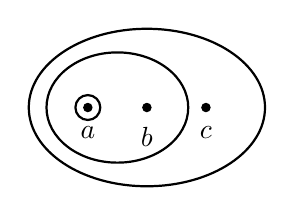
\begin{tikzpicture}
		\draw[thick] (0,0) ellipse (1.5 and 1);
		\filldraw (-.75,0) circle (1.5pt) node[label=below:$a$] 
		(a) {};
		\filldraw (0,0) circle (1.5pt) node[label=below:$b$] (b) 
		{};
		\filldraw (.75,0) circle (1.5pt) node[label=below:$c$] 
		(c) {};
		
		\draw[thick] (a) circle (4.5pt);
		\draw[thick] (-.375,0) ellipse (.9 and .7);
		\end{tikzpicture}
		\caption{These subsets are a topology for $X = \{ a, b, c 
		\}$.}\label{top example}
	\end{subfigure}
	\begin{subfigure}{2in}
		\centering
		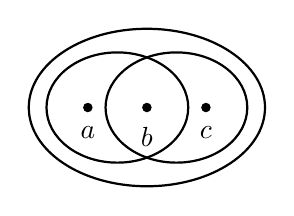
\begin{tikzpicture}
		\draw[thick] (0,0) ellipse (1.5 and 1);
		\filldraw (-.75,0) circle (1.5pt) node[label=below:$a$] 
		(a) {};
		\filldraw (0,0) circle (1.5pt) node[label=below:$b$] (b) 
		{};
		\filldraw (.75,0) circle (1.5pt) node[label=below:$c$] 
		(c) {};
		
		\draw[thick] (-.375,0) ellipse (.9 and .7);
		\draw[thick] (.375,0) ellipse (.9 and .7);
		\end{tikzpicture}
		\caption{These subsets are not a topology for $X = \{ a, 
		b, c \}$.}\label{top nonexample}
	\end{subfigure}
\end{marginfigure}

This is an extremely abstract definition, but the notion of open 
sets will lead to a definition of continuity: a 
generalization of the epsilon-delta definition from analysis. 
(See Section \ref{cont f sect}.) A given set will have more than 
one topology it 
can be equipped with.

\begin{example}
	If $X$ is any set, the collection of all subsets of $X$ is a 
	topology on $X$; it is called the \df{discrete 
	topology}\index{topology!discrete topology}. The collection 
	consisting of $X$ and $\varnothing$ only is also a topology 
	on $X$; it is called the \df{indiscrete 
	topology}\index{topology!indiscrete topology}, or the 
	\df{trivial topology}\index{topology!trivial topology}.
\end{example}

\begin{theorem}
	Let $X$ be a topological space. Then the following conditions 
	hold:
	\begin{enumerate}
		\item[(1)] $\varnothing$ and $X$ are closed.
		
		\item[(2)] Arbitrary intersections of closed sets are 
		closed.
		
		\item[(3)] Finite unions of closed sets are closed.
	\end{enumerate}
\end{theorem}

A bijective correspondence which preserves the topological 
structure is called a homeomorphism. See section 
\ref{homeomorphism}.

%%%%%%%%%%%%%%%%%%%%%%%%%%%%%%%%%%%%%%%%%%%%%%%%%%%%%%%%%%%%%%%%%%

\subsection{Comparing Topologies}

\begin{itemize}
	\item If $\ms{T} \subseteq \ms{T}'$, we say that $\ms{T}'$ is 
	\df{finer}\index{topology!finer} than $\ms{T}$. If $\ms{T} 
	\subsetneq \ms{T}'$, we say that $\ms{T}'$ is \df{strictly 
	finer} than $\ms{T}$. We also say that $\ms{T}$ is (strictly) 
	\df{coarser}\index{topology!coarser} than $\ms{T}'$. $\ms{T}$ 
	and $\ms{T}'$ are \df{comparable}\index{topology!comparable} 
	if $\ms{T} \subseteq \ms{T}'$ or $\ms{T}' \subseteq \ms{T}$.
	
	\item The statement ``$\ms{T}'$ is finer than $\ms{T}$'' is 
	equivalent to the statement ``For each $x \in X$ and each 
	basis element $B \in \ms{B}$ containing $x$, there is a basis 
	element $B' \in \ms{B}'$ such that $x \in B' \subseteq B$.''
\end{itemize}

%%%%%%%%%%%%%%%%%%%%%%%%%%%%%%%%%%%%%%%%%%%%%%%%%%%%%%%%%%%%%%%%%%

\subsection{Generating a Topology}

\begin{definition}[Basis For a Topology]\label{basis top}
	If $X$ is a set, a \df{basis}\index{topology!basis for a} for 
	a topology on $X$ is a collection $\ms{B}$ of subsets of $X$ 
	(called \df{basis elements}) such that
	\begin{enumerate}
		\item[(1)] For each $x \in X$, there is at least one 
		basis element $B$ containing $x$.
		
		\item[(2)] If $x$ belongs to the intersection of two 
		basis elements $B_1$ and $B_2$, then there is a basis 
		element $B_3$ containing $x$ such that $B_3 \subseteq B_1 
		\cap B_2$.
	\end{enumerate}
	If $\ms{B}$ satisfies these two conditions, we define the 
	\df{topology $\ms{T}$ generated by $\ms{B}$} as follows: A 
	subset $U$ of $X$ is open in $X$ if for each $x \in U$, there 
	is a basis element $B \in \ms{B}$ such that $x \in B$ and $B 
	\subseteq U$. Note that each basis element is itself an 
	element of $\ms{T}$.
\end{definition}

\begin{example}If $\ms{B}$ is the collection of all open 
intervals in the real line, the topology generated by $\ms{B}$ is 
called the \df{standard topology}\index{topology!standard 
topology of the real line} of the real line.
\end{example}

\begin{marginfigure}
	\centering
	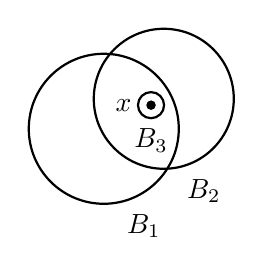
\begin{tikzpicture}
	\node[draw,thick,circle,minimum 
	size=.75in,label={[xshift=.2in]below:$B_1$}] at (0,0) {};
	
	\node[draw,thick,circle,minimum 
	size=.7in,label={[xshift=.2in]below:$B_2$}] at 
	(.3in,.15in) {};
	
	\filldraw (.6,.3) circle (1.5pt) node[label=left:$x$] 
	(x) {};
	\node[draw,circle,thick,label=below:$B_3$] at (.6,.3) 
	{};
	\end{tikzpicture}
	\caption{Illustration of condition (2) of Definition 
		\ref{basis top}}\label{cond 2 fig}
\end{marginfigure}

\begin{itemize}
	\item Let $X$ be a set; let $\ms{B}$ be a basis for a 
	topology $\ms{T}$ on $X$. Then $\ms{T}$ equals the collection 
	of all unions of elements of $\ms{B}$. That is, every open 
	set $U$ in $X$ can be expressed as a union of basis elements.
	
	\item We can obtain a basis for a given topology as follows: 
	Gather a collection $\ms{C}$ of open sets $U$ of $X$ such 
	that for each $x \in U$, there is an element $C$ of $\ms{C}$ 
	such that $x \in C \subseteq U$. $\ms{C}$ is a basis for the 
	topology of $X$.
\end{itemize}

	A \df{subbasis}\index{topology!subbasis} $\ms{S}$ is a 
	collection of subsets of $X$ whose union equals $X$. The 
	\df{topology generated by the subbasis} $\ms{S}$ is defined 
	to be the collection $\ms{T}$ of all unions of finite 
	intersections of elements of $\ms{S}$.
	

%%%%%%%%%%%%%%%%%%%%%%%%%%%%%%%%%%%%%%%%%%%%%%%%%%%%%%%%%%%%%%%%%%
%%%%%%%%%%%%%%%%%%%%%%%%%%%%%%%%%%%%%%%%%%%%%%%%%%%%%%%%%%%%%%%%%%

\newpage

\section{Closed Sets}

\begin{definition}[Closed Set]
	A subset $A$ of a topological space $X$ is said to be 
	\df{closed}\index{topology!closed set} if the set $X 
	\setminus A$ is open.
\end{definition}

A set can be both open and closed, one and not the 
other, or neither.
There are analogous theorems/definitions for closed sets as for 
open sets, and these have been placed alongside the 
theorems/definitions for open sets.

\begin{definition}[Interior and Closure of Set]
	Given a subset $A$ of a topological space, the 
	\df{interior}\index{topology!interior} of $A$ is defined as 
	the union of all open sets contained in $A$, and the 
	\df{closure}\index{topology!closure} of $A$ is defined as the 
	intersection of all closed sets containing $A$. The interior 
	of $A$ is denoted $\Int{A}$, and the closure of $A$ is 
	denoted by $\Cl{A}$ or $\bar{A}$.
\end{definition}

The main idea is that the closure of an open interval is a closed 
interval and the interior of a closed interval is an open 
interval.

\begin{itemize}
	\item We have $\Int{A} \subseteq A \subseteq \bar{A}$.
	
	\item If $A$ is open, $A = \Int{A}$; while if $A$ is closed, 
	$A = \bar{A}$.
\end{itemize}

\begin{theorem}
	Let $A$ be a subset of the topological space $X$.
	\begin{enumerate}
		\item[(a)] Then $x \in \bar{A}$ if and only if every 
		neighborhood of $x$ intersects $A$.
		
		\item[(b)] Supposing the topology of $X$ is given by a 
		basis, then $x \in \bar{A}$ if and only if every basis 
		element $B$ containing $x$ intersects $A$.
	\end{enumerate}
\end{theorem}

\begin{marginfigure}
	\centering
	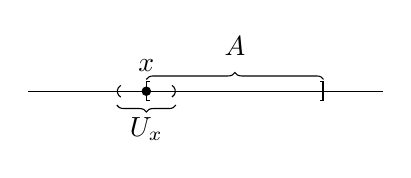
\begin{tikzpicture}[scale=1.5]
		\draw (0,0) -- (3,0);
		
		\draw[{Bracket[width=2.5mm]}-{Bracket[width=2.5mm]}] 
		(1,0) -- 
		(2.5,0);
		\filldraw (1,0) circle (1pt) node[label=above:$x$] (x) 
		{};
		\draw[decoration={brace},decorate] 
		(1,.1) -- node[above=5pt] {$A$} (2.5,.1);
		
		\draw[{Parenthesis-Parenthesis}] (.75,0) -- (1.25,0);
		\draw[decoration={brace,mirror,raise=5pt},decorate] 
		(.75,0) -- node[below=6pt] {$U_x$} (1.25,0);
	\end{tikzpicture}\caption{Any neighborhood of $x$ intersects 
	$A$, so $x \in \bar{A}$.}\label{th 321 a}
\end{marginfigure}

Part (a) is illustrated in Figure \ref{th 321 a}.

\begin{definition}[Limit Point]
	If $A$ is a subset of the topological space $X$ and if $x$ is 
	a point of $X$, we say that $x$ is a \df{limit 
	point}\index{topology!limit point} of $A$ if every 
	neighborhood of $x$ intersects $A$ in some point other than 
	$x$ itself. Equivalently, $x$ is a limit point of $A$ if it 
	belongs to the closure of $A \setminus \{ x \}$.
\end{definition}

The point $x$ may lie in $A$ or not.

\begin{theorem}
	Let $A$ be a subset of the topological space $X$; let $A'$ be 
	the set of all limit points of $A$. Then
	\[
		\bar{A} = A \cup A'\,.
	\]
\end{theorem}
	
\begin{corollary}
	A subset of a topological space is closed if and only if 
	it contains all its limit points.
\end{corollary}

\begin{theorem}
	Let $X$ be a space satisfying the $T_1$ axiom; let $A$ be a 
	subset of $X$. Then the point $x$ is a limit point of $A$ if 
	and only if every neighborhood of $x$ contains infinitely 
	many points of $A$.
\end{theorem}

\begin{theorem}
	Let $\{ X_\alpha \}$ be an indexed family of spaces; let 
	$A_\alpha \subseteq X_\alpha$ for each $\alpha$. If $\prod 
	X_\alpha$ is given either the product or the box topology, then
	\[
		\prod \bar{A}_\alpha = \overline{\prod A_\alpha}\,.
	\]
\end{theorem}

%%%%%%%%%%%%%%%%%%%%%%%%%%%%%%%%%%%%%%%%%%%%%%%%%%%%%%%%%%%%%%%%%%
%%%%%%%%%%%%%%%%%%%%%%%%%%%%%%%%%%%%%%%%%%%%%%%%%%%%%%%%%%%%%%%%%%

\newpage

\section{Important Topologies}

\subsection{The Order Topology}

\begin{definition}[Order Topology]
	Let $X$ be a set with a simple order relation; assume $X$ has 
	more than one element. Let $\ms{B}$ be the collection of all 
	sets of the following types: 
	\begin{enumerate}
		\item[(1)] All open intervals $(a,b)$ in $X$.
		
		\item[(2)] All intervals of the form $[a_0,b)$, where 
		$a_0$ is the smallest element (if any) of $X$.
		
		\item[(3)] All intervals of the form $(a,b_0]$, where 
		$b_0$ is the largest element (if any) of $X$.
	\end{enumerate}
	The collection $\ms{S}$ is a basis for a topology on $X$ 
	which is called the \df{order topology}\index{topology!order 
	topology}.
\end{definition}

\begin{example}
	The standard topology on $\reals$ is just the order topology 
	derived from the usual order on $\reals$.
\end{example}

The collection
\[
	\ms{B} = \{ (a,+\infty), (-\infty,b) \mid a,b \in X \}
\]
forms a subbasis for the order topology on $X$.

%%%%%%%%%%%%%%%%%%%%%%%%%%%%%%%%%%%%%%%%%%%%%%%%%%%%%%%%%%%%%%%%%%

\newpage

\subsection{The Box Topology}

\begin{definition}[Box Topology]
	Let $\{ X_\alpha \}_{\alpha \in J}$ be an indexed family of 
	topological spaces. Let us take as a basis for a topology on 
	the product space
	\[
		\prod_{\alpha \in J} X_\alpha
	\]
	the collection of all sets of the form
	\[
		\prod_{\alpha \in J} U_\alpha\,,
	\]
	where $U_\alpha$ is open in $X_\alpha$ for each $\alpha \in J$. 
	The topology generated by this basis is called the \df{box 
	topology}\index{topology!box topology}.
\end{definition}

\begin{marginfigure}
	\centering
	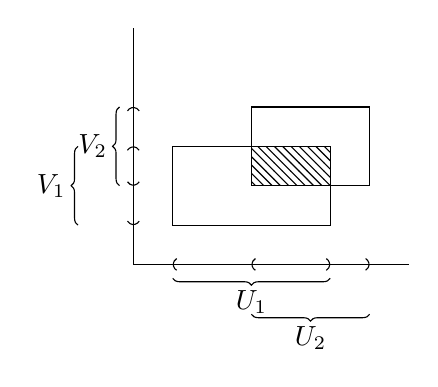
\begin{tikzpicture}
		\draw (0,0) -- (0,3);
		
		\draw (0,0) -- (3.5,0);
		
		\draw (.5,.5) rectangle (2.5,1.5);
		
		\draw (1.5,1) rectangle (3,2);
		
		\draw[pattern=north west lines] (1.5,1) rectangle 
		(2.5,1.5);
		
		\draw[{Parenthesis-Parenthesis}] (.5,0) -- (2.5,0);
		\draw[decoration={brace,mirror,raise=5pt},decorate] 
		(.5,0) -- node[below=6pt] {$U_1$} (2.5,0);
		
		\draw[{Parenthesis-Parenthesis}] (1.5,0) -- (3,0);
		\draw[decoration={brace,mirror,raise=18pt},decorate] 
		(1.5,0)	-- node[below=19pt] {$U_2$} (3,0);
		
		\draw[{Parenthesis-Parenthesis}] (0,.5) -- (0,1.5);
		\draw[decoration={brace,raise=20pt},decorate] 
		(0,.5)	-- node[left=21pt] {$V_1$} (0,1.5);
		
		\draw[{Parenthesis-Parenthesis}] (0,1) -- (0,2);
		\draw[decoration={brace,raise=5pt},decorate] 
		(0,1)	-- node[left=6pt] {$V_2$} (0,2);
	\end{tikzpicture}\caption{Condition 2 for a 
	basis.}\label{box space condition 2}
\end{marginfigure}

Figure \ref{box space condition 2} illustrates that the 
second condition for a basis is met. We prefer the product topology 
over the box topology.

\begin{theorem}
	Suppose the topology on each space $X_\alpha$ is given by a 
	basis $\ms{B}_\alpha$. The collection of all sets of the form 
	$\prod_{\alpha \in J} B_\alpha$, where $B_\alpha \in 
	\ms{B}_\alpha$ for each $\alpha$, will serve as a basis for the 
	box topology on $\prod_{\alpha \in J} X_\alpha$.
\end{theorem}

The box topology turns out to be less useful than the product 
topology, so that one will be used.

%%%%%%%%%%%%%%%%%%%%%%%%%%%%%%%%%%%%%%%%%%%%%%%%%%%%%%%%%%%%%%%%%%

\newpage

\subsection{The Product Topology}

\begin{definition}[Product Topology]
	Let $\ms{S}_\beta$ denote the collection
	\[
		\ms{S}_\beta = \{ \pi_\beta^{-1}(U_\beta) \mid U_\beta 
		\text{ 
		is open in } X_\beta \}\,,
	\]
	and let $\ms{S}$ denote the union of these collections,
	\[
		\ms{S} = \bigcup_{\beta \in J} \ms{S}_\beta\,.
	\]
	The topology generated by the subbasis $\ms{S}$ is called the 
	\df{product topology}\index{topology!product topology}. In this 
	topology $\prod_{\alpha \in J} X_\alpha$ is called a 
	\df{product space}\index{topology!product space}.
\end{definition}

\begin{marginfigure}
	\centering
	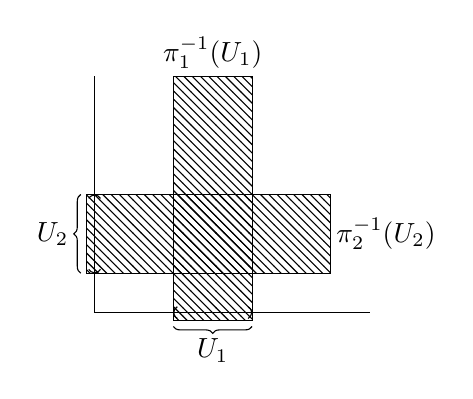
\begin{tikzpicture}
	\draw (0,0) -- (0,3);
	
	\draw (0,0) -- (3.5,0);
	
	\draw[pattern=north west lines] (1,-.1) rectangle (2,3);
	
	\node at (1.5,3.3) {$\pi_1^{-1}(U_1)$};
	
	\draw[{Parenthesis-Parenthesis}] (1,0) -- (2,0);
	\draw[decoration={brace,mirror,raise=5pt},decorate] 
	(1,0)	-- node[below=6pt] {$U_1$} (2,0);
	
	\draw[{Parenthesis-Parenthesis}] (0,.5) -- (0,1.5);
	\draw[decoration={brace,raise=5pt},decorate] 
	(0,.5)	-- node[left=6pt] {$U_2$} (0,1.5);
	
	\draw[pattern=north west lines] (-.1,.5) rectangle (3,1.5);
	
	\node at (3.7,1) {$\pi^{-1}_2(U_2)$};
	\end{tikzpicture}\caption{Illustration of the subbasis of the 
	product topology for $U_1 \times U_2$.}\label{prod subbasis}
\end{marginfigure}

Figure \ref{prod subbasis} illustrates this definition.

A typical element of the basis generated by $\ms{S}$ has the form
\[
	B = \pi_{\beta_1}^{-1}(U_{\beta_1}) \cap 
	\pi_{\beta_2}^{-1}(U_{\beta_2}) \cap 
	\dots \cap 
	\pi_{\beta_n}^{-1}(U_{\beta_n})
\]
for distinct $\beta_i$, and therefore we have the following theorem.

\begin{theorem}
	The product topology on $\prod 	X_\alpha$ has as basis all sets 
	of the form $\prod U_\alpha$, where $U_\alpha$ is open in 
	$X_\alpha$ for each $\alpha$ and $U_\alpha$ equals $X_\alpha$ 
	except for finitely many values of $\alpha$.
\end{theorem}

\begin{theorem}
	Suppose the topology on each space $X_\alpha$ is given by a 
	basis $\ms{B}_\alpha$. The collection of all sets of the form 
	$\prod_{\alpha \in J} B_\alpha$, where $B_\alpha \in 
	\ms{B}_\alpha$ for finitely many indices $\alpha$ and $B_\alpha 
	= X_\alpha$ for all the remaining indices, will serve as a 
	basis for the product topology $\prod_{\alpha \in J} X_\alpha$.
\end{theorem}

%%%%%%%%%%%%%%%%%%%%%%%%%%%%%%%%%%%%%%%%%%%%%%%%%%%%%%%%%%%%%%%%%%

\newpage

\subsection{The Subspace Topology}

\begin{definition}[Subspace Topology]
	Let $X$ be a topological space with topology $\ms{T}$. If $Y$ 
	is a subset of $X$, the collection
	\[
		\ms{T}_Y = \{ Y \cap U \mid U \in \ms{T} \}
	\]
	is a topology on $Y$, called the \df{subspace 
	topology}\index{topology!subspace topology}. With this 
	topology, $Y$ 
	is called a \df{subspace}\index{topology!subspace} of $X$.
\end{definition}

If $\ms{B}$ is a basis for the topology of $X$ then the collection
\[
	\ms{B}_Y = \{ B \cap Y \mid B \in \ms{B} \}
\]
is a basis for the subspace topology on $Y$.

\begin{theorem}		
	Let $Y$ be a subspace of $X$. Then a set $A$ is 
	closed in $Y$ if and only if it equals the intersection 
	of a closed set of $X$ with $Y$.
\end{theorem}

\begin{theorem}
	$ $
	\begin{itemize}
		\item Let $Y$ be a subspace of $X$. If $U$ is open in $Y$ 
		and $Y$ is open in $X$, then $U$ is open in $X$.
		
		\item Let $Y$ be a subspace of $X$. If $A$ is closed in 
		$Y$ and $Y$ is closed in $X$, then $A$ is closed in $X$.
	\end{itemize}
\end{theorem}

\begin{theorem}
	Let $Y$ be a subspace of $X$; let $A$ be a subset of $Y$; let 
	$\bar{A}$ denote the closure of $A$ in $X$. Then the closure 
	of $A$ in $Y$ equals $\bar{A} \cap Y$.
\end{theorem}

%%%%%%%%%%%%%%%%%%%%%%%%%%%%%%%%%%%%%%%%%%%%%%%%%%%%%%%%%%%%%%%%%%

\newpage

\subsection{Metrics and The Metric Topology}

Main Idea: A metric is a way to measure distance. The metric 
topology is the collection of open balls, a generalization of the 
open interval. It really belongs to the field of analysis rather 
than topology.

\begin{definition}[Metric]
	A \df{metric}\index{topology!metric} on a set $X$ is a function 
	$d: X \times X \to \reals$ having the following properties:
	\begin{enumerate}
		\item $d(xy) \geq 0$ for all $x,y \in X$; equality holds if 
		and only if $x = y$.
		
		\item $d(x,y) = d(y,x)$ for all $x,y \in X$.
		
		\item (Triangle Inequality) $d(x,y) + d(y,z) \geq d(x,z)$, 
		for all $x,y,z \in X$.
	\end{enumerate}
\end{definition}

\begin{definition}[$\epsilon$-Ball]
	Given a metric $d$ on $X$, the number $d(x,y)$ is often called 
	the \df{distance} between $x$ and $y$ in the metric $d$. Given 
	$\epsilon > 0$, consider the set
	\[
		B_d(x,\epsilon) = \{ y \mid d(x,y) < \epsilon \}
	\]
	of all points $y$ whose distance from $x$ is less than 
	$\epsilon$. It is called the \df{$\epsilon$-ball centered at 
	$x$}\index{topology!$\epsilon$-ball}.
\end{definition}

\begin{definition}[Metric Topology]
	If $d$ is a metric on the set $x$, then the collection of all 
	$\epsilon$-balls $B_d(x,\epsilon)$, for $x \in X$ and $\epsilon 
	> 0$, is a basis for a topology on $X$, called the \df{metric 
	topology}\index{topology!metric topology} induced by $d$.
\end{definition}

A set $U$ is open in the metric topology induced by $d$ if and only 
if for each $y \in U$, there is a $\delta > 0$ such that 
$B_d(y,\delta) \subseteq U$.

%%%%%%%%%%%%%%%%%%%%%%%%%%%%%%%%%%%%%%%%%%%%%%%%%%%%%%%%%%%%%%%%%%

\subsubsection{Relevant Definitions}

\begin{itemize}
	\item If $X$ is a topological space, $X$ is said to be 
	\df{metrizable}\index{topology!metrizable} if there exists a 
	metric $d$ on the set $X$ which induces the topology of $X$. A 
	\df{metric space}\index{topology!metric space} is a metrizable 
	space $X$ together with a specific metric $d$ that gives the 
	topology of $X$.
	
	\item Let $X$ be a metric space with metric $d$. A subset $A$ 
	of $X$ is said to be \df{bounded} if there is some number $M$ 
	such that
	\[
		d(a_1,a_2) \leq M
	\]
	for every pair $a_1$, $a_2$ of points of $A$. If $A$ is bounded 
	and nonempty, the \df{diameter} of $A$ is defined to be the 
	number 
	\[
		\diam A = \sup \{ d(a_1,a_2) \mid a_1,a_2 \in A \}\,.
	\]
	
	\item Given $\bt{x} = (x_1, \dots, x_n)$ in $\reals^n$, we 
	define the \df{norm} of \bt{x} by the equation 
	\[
		\| \bt{x} \| = (x_1^2 + \dots + x_n^2)^{1/2}\,.
	\]
\end{itemize}
	
Remark: Metrizability is always a highly desirable attribute for a 
space to possess, for the existence of a metric gives one a 
valuable tool for proving theorems about the space. Though 
Metrizability is a topological property, properties that involve a 
specific metric for $X$ in general do not.

$\reals^\omega$ equipped with the metric topology is metrizable:

\begin{theorem}
	Let $\bar{d}(a,b) = \min \{ |a-b|, 1 \}$ be the standard 
	bounded metric on $\reals$. If \bt{x} and \bt{y} are two points 
	of $\reals^\omega$, define
	\[
		D(\bt{x}, \bt{y}) = \sup \left\{ \frac{\bar{d}(x_i,y_i)}{i} 
		\right\}\,.
	\]
	Then $D$ is a metric that induces the product topology on 
	$\reals^\omega$.
\end{theorem}

%%%%%%%%%%%%%%%%%%%%%%%%%%%%%%%%%%%%%%%%%%%%%%%%%%%%%%%%%%%%%%%%%%

\subsubsection{Important Metrics}

\begin{itemize}
	\item The standard metric on the real numbers $\reals$ is 
	defined by the equation $d(x,y) = | x-y |$. It induces the 
	order topology. Thus, $\reals$ with the standard topology is 
	metrizable, and $\reals$ with the standard topology and the 
	standard metric form a metric space. In fact $\reals^n$ and 
	$\reals^\omega$ are 
	metrizable.
	
	\item Let $X$ be a metric space with metric $d$. Define 
	$\bar{d} : X \times X \to \reals$ by the equation $\bar{d}(x,y) 
	= \min \{ d(x,y), 1 \}$. $\bar{d}$ is called the \df{standard 
	bounded metric} corresponding to $d$, and induces the same 
	topology as $d$.
	
	\item We define the \df{euclidean metric} $d$ on $\reals^n$ by 
	the equation
	\[
		d(\bt{x},\bt{y}) = \| \bt{x} - \bt{y} \|
			= [(x_1 - y_1)^2 + \dots + (x_n - y_n)^2]^{1/2}\,.
	\]
	$d$ induces the product topology on $\reals^n$.
	In $\reals^2$, the basis elements under $d$ can be pictured as 
	circular regions.
	
	\item We define the \df{square metric} $\rho$ by the equation
	\[
		\rho(\bt{x},\bt{y}) = \max \{ |x_1-y_1|, \dots, |x_n-y_n| 
		\}\,.
	\]
	$\rho$ induces the product topology on $\reals^n$.
	In $\reals^2$, the basis elements under $\rho$ can be pictured 
	as square regions.
	
	\item Given an index set $J$, and given points $\bt{x} = 
	(x_\alpha)_{\alpha \in J}$ and $\bt{y} = (y_\alpha)_{\alpha \in 
	J}$ of $\reals^J$, let us define a metric $\bar{\rho}$ on 
	$\reals^J$ by the equation
	\[
		\bar{\rho}(\bt{x},\bt{y}) = \sup \{ \bar{d} 
		(x_\alpha,y_\alpha) \mid \alpha \in J \}\,,
	\]
	where $\bar{d}$ is the standard bounded metric on $\reals$. 
	$\bar{\rho}$ is called the \df{uniform metric} on $\reals^J$, 
	and the topology it induces is called the \df{uniform topology}.
\end{itemize}

%%%%%%%%%%%%%%%%%%%%%%%%%%%%%%%%%%%%%%%%%%%%%%%%%%%%%%%%%%%%%%%%%%

\newpage

\subsection{Relationships Between Important Topologies}

The box and product topologies are equivalent when acting on a 
finite Cartesian product, but not on an arbitrary Cartesian 
product. We prefer the product topology.

\begin{theorem}
	Let $A_\alpha$ be a subspace of $X_\alpha$ for each $\alpha \in 
	J$. Then $\prod A_\alpha$ is a subspace of $\prod X_\alpha$ if 
	both products are given the box topology, or if both products 
	are given the product topology.
\end{theorem}

Let $X$ be an ordered set in the order topology, and let $Y$ be a 
subset of $X$. The order relation on $X$, when restricted to $Y$, 
makes $Y$ into an ordered set. However, the resulting order 
topology on $Y$ need not be the same as the topology that $Y$ 
inherits as a subspace of $X$. The following theorem tells us 
when they are the same, but we need a definition first.

\begin{definition}[Convex]
	Given an ordered set $X$, let us say that a subset $Y$ of $X$ 
	is \df{convex}\index{topology!convex} in $X$ if for each air 
	of points 
	$a < b$ of $Y$, the entire interval $(a,b)$ of points of $X$ 
	lies in $Y$.
\end{definition}

\begin{theorem}
	Let $X$ be an ordered set in the order topology; let $Y$ be a 
	subset of $X$ that is convex in $X$. Then the order topology 
	on $Y$ is the same as the topology $Y$ inherits as a subspace 
	of $X$.
\end{theorem}

\begin{theorem}
	The uniform topology on $\reals^J$ is finer than the product 
	topology and coarser than the box topology; these three 
	topologies are all different if $J$ is infinite.
\end{theorem}

%%%%%%%%%%%%%%%%%%%%%%%%%%%%%%%%%%%%%%%%%%%%%%%%%%%%%%%%%%%%%%%%%%
%%%%%%%%%%%%%%%%%%%%%%%%%%%%%%%%%%%%%%%%%%%%%%%%%%%%%%%%%%%%%%%%%%

\newpage

\section{Hausdorff Spaces}

Topological spaces in which one-point sets are not closed are 
strange and rare in other branches of mathematics. Therefore, we 
usually consider a class of spaces called Hausdorff spaces, which 
exclude such cases.

\begin{definition}[Hausdorff Space]
	A topological space $X$ is called a \df{Hausdorff 
	space}\index{topology!Hausdorff} if for each pair $x_1, x_2$ 
	of distinct points of $X$, there exist neighborhoods $U_1$ 
	and $U_2$ of $x_1$ and $x_2$, respectively, that are disjoint.
\end{definition}

\begin{marginfigure}
	\centering
	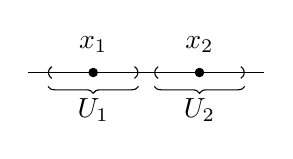
\begin{tikzpicture}
	\draw (0,0) -- (3,0);
	\filldraw (.825,0) circle (1.5pt) node[label=above:$x_1$] 
	(x1) {};
	\draw[{Parenthesis-Parenthesis}] (.25,0) -- (1.4,0);
	\draw[decoration={brace,mirror,raise=5pt},decorate] 
	(.25,0) -- node[below=6pt] {$U_1$} (1.4,0);
	
	\filldraw (2.175,0) circle (1.5pt) 
	node[label=above:$x_2$] 
	(x2) {};
	\draw[{Parenthesis-Parenthesis}] (1.6,0) -- (2.75,0);
	\draw[decoration={brace,mirror,raise=5pt},decorate] 
	(1.6,0) -- node[below=6pt] {$U_2$} (2.75,0);
	\end{tikzpicture}
	\caption{The real line equipped with the standard topology is 
	Hausdorff.}\label{real line hausdorff}
\end{marginfigure}

Figure \ref{real line hausdorff} illustrates the notion of a 
Hausdorff space using $\reals$ as an example. Given $x_1$ and 
$x_2$, it is always possible to find such a $U_1$ and $U_2$. Note 
that a different topology on $\reals$ (for example the finite 
complement topology) may not be Hausdorff.

\begin{theorem}
	Every finite point set in a Hausdorff space $X$ is closed.
\end{theorem}

The Hausdorff condition is stronger than the condition that 
finite point sets be closed, which is called the $T_1$ axiom. See 
Section \ref{ti axioms}.

\begin{theorem}
	Every simply ordered set is a Hausdorff space in the order 
	topology. If each space $X_\alpha$ is a Hausdorff space, then 
	$\prod X_\alpha$ is a Hausdorff space in both the box and 
	product topologies. A subspace of a Hausdorff space is a 
	Hausdorff space.
\end{theorem}


%%%%%%%%%%%%%%%%%%%%%%%%%%%%%%%%%%%%%%%%%%%%%%%%%%%%%%%%%%%%%%%%%%
%%%%%%%%%%%%%%%%%%%%%%%%%%%%%%%%%%%%%%%%%%%%%%%%%%%%%%%%%%%%%%%%%%

\newpage

\section{Sequences (Topology)}

\begin{definition}[Convergence of a Sequence]
	Let $X$ be a topological space. A sequence $x_1, x_2, \dots$ of 
	points in $X$ \df{converges}\index{topology!converging 
		sequence} to the point $x$ of $X$ provided that, 
	corresponding to each neighborhood $U$ of $x$, there is a 
	positive integer $N$ such that $x_n \in U$ for all $n \geq 
	N$. If the sequence $x_n$ of points of the Hausdorff space 
	$X$ converges to the point $x$ of $X$, we often write $x_n 
	\to x$, and we say that $x$ is the 
	\df{limit}\index{topology!limit of sequence} of the sequence 
	$x_n$.
\end{definition}

\begin{marginfigure}
	\centering
	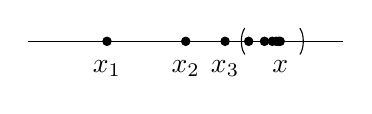
\begin{tikzpicture}
		\draw (0,0) -- (4,0);
		
		\filldraw (1,0) circle (1.5pt) node[label=below:$x_1$] 
		(x1) {};
		\filldraw (2,0) circle (1.5pt) node[label=below:$x_2$] (x2) 
		{};
		\filldraw (2.5,0) circle (1.5pt) node[label=below:$x_3$] 
		(x3) {};
		\filldraw (2.8,0) circle (1.5pt);
		\filldraw (3,0) circle (1.5pt);
		\filldraw (3.1,0) circle (1.5pt);
		\filldraw (3.15,0) circle (1.5pt);
		\filldraw (3.18,0) circle (1.5pt);
		\filldraw (3.2,0) circle (1.5pt) node[label=below:$x$] (x) 
		{};
		\draw[{Parenthesis[width=4mm]}-{Parenthesis[width=4mm]}] 
		(2.7,0) -- (3.5,0);
	\end{tikzpicture}
	\caption{Any neighborhood of $x$ contains all but a finite 
	number of points of the sequence $x_n$ and so is a limit of the 
	sequence $x_n$.}\label{conv seq}
\end{marginfigure}

Note that if any neighborhood of $x$ contains all but a finite 
number of points of the sequence, then there must necessarily be 
some $N$ such that $x_n$ belongs to the neighborhood for $n \geq 
N$. Figure \ref{conv seq} illustrates this view.

\begin{theorem}
	If $X$ is a Hausdorff space, then a sequence of points of $X$ 
	converges to at most one point of $X$.
\end{theorem}

%%%%%%%%%%%%%%%%%%%%%%%%%%%%%%%%%%%%%%%%%%%%%%%%%%%%%%%%%%%%%%%%%%
%%%%%%%%%%%%%%%%%%%%%%%%%%%%%%%%%%%%%%%%%%%%%%%%%%%%%%%%%%%%%%%%%%

\newpage

\section{$T_i$ Axioms}\label{ti axioms}

\begin{definition}[$T_i$ Axioms]
	$ $
	\begin{itemize}
		\item The condition that finite point sets be closed is 
		called the \df{$T_1$ axiom}\index{topology!$T_1$ axiom}.
	\end{itemize}
\end{definition}

The $T_1$ axiom is too weak to prove many of the interesting 
theorems of topology, so we rely on the Hausdorff condition.

%%%%%%%%%%%%%%%%%%%%%%%%%%%%%%%%%%%%%%%%%%%%%%%%%%%%%%%%%%%%%%%%%%
%%%%%%%%%%%%%%%%%%%%%%%%%%%%%%%%%%%%%%%%%%%%%%%%%%%%%%%%%%%%%%%%%%

\newpage

\section{Continuous Function}\label{cont f sect}

\begin{definition}[Continuous Function]
	Let $X$ and $Y$ be topological spaces. A function $f:X \to Y$ 
	is said to be \df{continuous}\index{topology!continuous 
	function} if for each open subset $V$ of 
	$Y$, the set $f^{-1}(V)$ is an open subset of $X$.
\end{definition}

In $\reals$, this definition is equivalent to the epsilon-delta 
definition of the continuity of a function; however, the 
topological definition includes other spaces and situations as 
well.

%%%%%%%%%%%%%%%%%%%%%%%%%%%%%%%%%%%%%%%%%%%%%%%%%%%%%%%%%%%%%%%%%%

\subsection{Demonstrating a Function Is Continuous}

\begin{itemize}
	\item If the topology of the range space $Y$ is given by a 
	basis $\ms{B}$, then to prove continuity of $f$ it suffices 
	to show that the inverse image of every basis element is open.
	
	\item If the topology on $Y$ is given by a subbasis $\ms{S}$, 
	to prove continuity of $f$ it suffices to show that the 
	inverse image of each subbasis element is open.
	
	\item $f:X \to Y$ is continuous if and only if for every 
	subset $A$ of $X$, one has $f(\bar{A}) \subseteq 
	\overline{f(A)}$.
	
	\item $f:X \to Y$ is continuous if and only if for every 
	closed set $B$ of $Y$, the set $f^{-1}(B)$ is closed in $X$.
	
	\item $f:X \to Y$ is continuous if and only if for each $x 
	\in X$ and each neighborhood $V$ of $f(x)$, there is a 
	neighborhood $U$ of $x$ such that $f(U) \subseteq V$. If this 
	condition holds for the point $x$ of $X$, we say that $f$ is 
	\df{continuous at the point $x$}.
\end{itemize}

%%%%%%%%%%%%%%%%%%%%%%%%%%%%%%%%%%%%%%%%%%%%%%%%%%%%%%%%%%%%%%%%%%

\subsection{Constructing Continuous Functions}

Let $X$, $Y$, and $Z$ be topological spaces.
\begin{itemize}
	\item (Constant function) If $f: X \to Y$ maps all of $X$ into 
	a single point $y_0$ of $Y$, then $f$ is continuous.
	
	\item (Inclusion) If $A$ is a subspace of $X$, the inclusion 
	function $j: A \to X$ is continuous.
	
	\item (Composites) If $f:X \to Y$ and $g:Y \to Z$ are 
	continuous, then the map $g \circ f:X \to Z$ is continuous.
	
	\item (Restricting the domain) If $f:X \to Y$ is continuous, 
	and if $A$ is a subspace of $X$, then the restricted function 
	$f|A:A \to Y$ is continuous.
	
	\item (Restricting or expanding the range) Let $f:X \to Y$ be 
	continuous. If $Z$ is a subspace of $Y$ containing the image 
	set $f(X)$, then the function $g:X \to Z$ obtained by 
	restricting the range of $f$ is continuous. If $Z$ is a space 
	having $Y$ as a subspace, then the function $h:X \to Z$ 
	obtained by expanding the range of $f$ is continuous.
	
	\item (Local formulation of continuity) The map $f:X \to Y$ is 
	continuous if $X$ can be written as the union of open sets 
	$U_\alpha$ such that $f|U_\alpha$ is continuous for each 
	$\alpha$.
\end{itemize}

\begin{theorem}[The Pasting Lemma]\index{topology!pasting lemma}
	Let $X = A \cup B$, where $A$ and $B$ are closed in $X$. Let 
	$f:A \to Y$ and $g:B \to Y$ be continuous. If $f(x) = g(x)$ for 
	every $x in A \cap B$, then $f$ and $g$ combine to give a 
	continuous function $h:X \to Y$, defined by setting $h(x) = 
	f(x)$ if $x \in A$, and $h(x) = g(x)$ if $x \in B$.
\end{theorem}
Remark: This theorem also holds if $A$ and $B$ are open sets in 
$X$; this is just a special case of the ``local formulation of 
continuity'' rule.

\begin{theorem}[Maps Into Products]
	Let $f:A \to \prod_{\alpha \in J} X_\alpha$ be given by the 
	equation $f(a) = (f_\alpha(a))_{\alpha \in J}$, where 
	$f_\alpha:A \to X_\alpha$ for each $\alpha$. Let $\prod 
	X_\alpha$ have the product topology. Then the function $f$ is 
	continuous if and only if each function $f_\alpha$ is 
	continuous.
\end{theorem}
Remark: The maps $f_1$ and $f_2$ are called the \df{coordinate 
functions}\index{topology!coordinate function} of $f$. Moreover, 
this theorem doesn't hold if one uses the box topology, which is 
one reason we prefer the product topology.

%%%%%%%%%%%%%%%%%%%%%%%%%%%%%%%%%%%%%%%%%%%%%%%%%%%%%%%%%%%%%%%%%%
%%%%%%%%%%%%%%%%%%%%%%%%%%%%%%%%%%%%%%%%%%%%%%%%%%%%%%%%%%%%%%%%%%

\newpage

\section{Homeomorphisms}\label{homeomorphism}

\begin{definition}[Homeomorphism]
	Let $X$ and $Y$ be topological spaces; let $f:X \to Y$ be a 
	bijection. If both the function $f$ and the inverse function 
	$f^{-1}:Y \to X$ are continuous, then $f$ is called a 
	\df{homeomorphism}\index{topology!homeomorphism}.
\end{definition}

What this really means is that $f$ is a homeomorphism if it is a 
bijective correspondence between the collections of open sets of 
$X$ and of $Y$. Thus, a homeomorphism is a bijective 
correspondence that preserves the topological structure involved.

\begin{marginfigure}
	\centering
	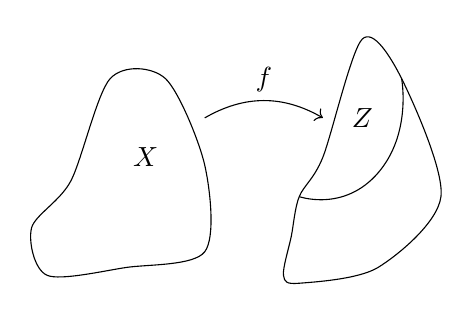
\begin{tikzpicture}
		\draw plot [smooth cycle] coordinates {(0,0) (1,0.1) 
		(2,0.3) (2,1.4) (1.5,2.5) (0.8,2.5) (0.3,1.2) (-0.2,0.6) } 
		node at (1.25,1.5) {$X$};
	
		\draw plot [smooth cycle] coordinates { (3,0) (3.1,.5) 
		(3.2,1) (3.5,1.5) (4,3) (4.5,2.5) (5,1) (4.2,.1) (3.2,-.1) 
		};
	
		\draw plot [smooth,tension=1.2] coordinates {(3.2,1) 
		(4.2,1.3) (4.5,2.5)} node at (4,2) {$Z$};
	
		\draw[->] (2,2) to [out=30,in=150] (3.5,2) node[above] at 
		(2.75,2.2) {$f$};
	\end{tikzpicture}
	\caption{If $f':X \to Z$ is a homeomorphism of $X$ with $Z$, 
	then $f'$ is a topological imbedding of $X$ in $Y$.}\label{top 
	imb}
\end{marginfigure}

\begin{definition}[Topological Imbedding]
	Suppose $f:X \to Y$ is an injective continuous map. Let $Z$ be 
	the image set $f(X)$, considered as a subspace of $Y$; then the 
	function $f':X \to Z$ obtained by restricting the range of $f$ 
	is bijective. If $f'$ happens to be a homeomorphism of $X$ with 
	$Z$, we say that the map $f:X \to Y$ is a \df{topological 
	imbedding}\index{topology!imbedding} of $X$ in $Y$.
\end{definition}

Figure \ref{top imb} illustrates this definition. Intuitively, the 
imbedding lets us treat $X$ as a subspace of $Y$ even though $X$ 
isn't a subset of $Y$.































	
\chapter{Analysis}

\chapter{Group Theory}

Abstract algebra is, as its name suggests, extremely abstract. It 
arose as an attempt to abstract the techniques used in algebraic 
equations, number theory, and geometry.
There are many specific examples of groups, and the power of the 
abstract point of view becomes apparent when results for all of 
these examples are obtained by providing a single result for the 
abstract group. The information in this chapter is based on Dummit 
and Foote's \emph{Abstract Algebra} (2004).

%%%%%%%%%%%%%%%%%%%%%%%%%%%%%%%%%%%%%%%%%%%%%%%%%%%%%%%%%%%%%%%%%%

\newpage

\section{Notation}

\begin{itemize}
	\item We write $ab$ for $a \cdot b$.
	
	\item We denote the identity element of an abstract group $(G, 
	\cdot)$ by 1.
	
	\item We denote $xx \dots x$ ($n$ terms) by $x^n$ and $x^{-1} 
	x^{-1} \dots x^{-1}$ ($n$ terms) by $x^{-n}$.
	
	\item When the operation is +, the identity will be denoted by 
	0, and for any element $a$, the inverse will be written $-a$. 
	Moreover, $a+ \dots + a$ ($n > 0$ terms) will be written $na$; 
	$-a - a \dots -a$ ($n$ terms) will be written $-na$ and $0a = 
	0$.
	
	\item For each $n \in \zplus$ let $GL_n(F)$ be the set of all 
	$n \times n$ matrices whose entries come from $F$ and whose 
	determinant is nonzero.
\end{itemize}

%%%%%%%%%%%%%%%%%%%%%%%%%%%%%%%%%%%%%%%%%%%%%%%%%%%%%%%%%%%%%%%%%%

\newpage

\section{Definition and Examples}

\begin{definition}[Binary Operation]
	$ $
	\begin{enumerate}
		\item A \df{binary operation}\index{group theory!binary 
		operation} $\cdot$ on a set $G$ is a function $\cdot : G 
		\times G \to G$. For any $a,b \in G$ we	write $a \cdot b$.
		
		\item A binary operation $\cdot$ on a set $G$ is 
		\df{associative}\index{group theory!associative} if for all 
		$a,b,c \in G$ we have $a \cdot (b \cdot c) = (a \cdot b) 
		\cdot c$.
		
		\item If $\cdot$ is a binary operation on a set $G$ we say 
		elements $a$ and $b$ of $G$ \df{commute}\index{group 
			theory!commutative} if $a \cdot b = b \cdot a$. We say 
		$\cdot$ (or $G$) is \df{commutative} if for all $a,b \in 
		G$, $a \cdot b = b \cdot a$.
		
		\item Suppose that $\cdot$ is a binary operation on a set 
		$G$ and $H$ is a subset of $G$. If the restriction of 
		$\cdot$ to $H$ is a binary operation on $H$, i.e., for all 
		$a,b \in H$, $a \cdot b \in H$, then $H$ is said to be 
		\df{closed}\index{group theory!closed under operation} 
		under $\cdot$.
	\end{enumerate}
\end{definition}

\begin{definition}[Group]
	$ $
	\begin{enumerate}
		\item A \df{group}\index{group theory!group} is an ordered 
		pair $(G,\cdot)$ where $G$ is a set and $\cdot$ is a binary 
		operation on $G$ satisfying the following axioms:
		\begin{enumerate}
			\item $\cdot$ is associative,
			
			\item there exists an element $e$ in $G$, called an 
			\df{identity}\index{group theory!identity element} of 
			$G$, such that for all $a \in G$ we have $a \cdot e = e 
			\cdot a = a$,
			
			\item for each $a \in G$ there is an element $a^{-1}$ 
			of $G$, called an \df{inverse}\index{group 
				theory!inverse of element} of $a$, such that $a 
				\cdot 
			a^{-1} = a^{-1} \cdot a = e$.
		\end{enumerate}
		
		\item The group $(G, \cdot)$ is called 
		\df{abelian}\index{group theory!abelian} (or 
		\df{commutative}\index{group theory!commutative group}) if 
		$a \cdot b = b \cdot a$ for all $a,b \in G$.
	\end{enumerate}
\end{definition}

Remark: We say $(G, \cdot)$ is a \df{finite group}\index{group 
theory!finite 
group} if in addition $G$ is a 
finite set.

\begin{example}
	$ $
	\begin{itemize}
		\item $\integers$, $\rationals$, $\reals$, and $\complex$ 
		are groups under + with $e = 0$ and $a^{-1} = -a$, for all 
		$a$.
		
		\item $\rationals \setminus \{ 0 \}$, $\reals \setminus \{ 
		0 \}$, $\complex \setminus \{ 0 \}$, $\rationals^+$, 
		$\reals^+$ are groups under $\times$ with $e = 1$ and 
		$a^{-1} = \frac{1}{a}$, for all $a$.
	\end{itemize}
\end{example}

%%%%%%%%%%%%%%%%%%%%%%%%%%%%%%%%%%%%%%%%%%%%%%%%%%%%%%%%%%%%%%%%%%

\newpage

\section{How to Form New Groups From Given Ones}

\begin{itemize}
	\item If $(A,\cdot)$ and $(B,*)$ are groups, we can form a new
	group $(A \times B, \diamond)$, called their \df{direct 
	product}\index{group theory!direct product}, whose elements are 
	those in the Cartesian product $A \times B$ and whose operation 
	is defined componentwise:
	\[
		(a_1,b_1)(a_2,b_2) = (a_1 \cdot a_2, b_1 * b_2)\,.
	\]

	\begin{example}
		If we take $A = B = \reals$ (both operations addition), 
		$\reals \times \reals$ is the familiar Euclidean plane.
	\end{example}

	\item Let $G$ be a group. The subset $H$ of $G$ is a 
	\df{subgroup}\index{group theory!subgroup} of $G$ if $H$ is 
	nonempty and $H$ is closed under products and inverses. If $H$ 
	is a subgroup of $G$ we shall write $H \leq G$.
	
	Remark: Subgroups of $G$ are just subsets of $G$ which are 
	themselves groups with respect to the operation defined in $G$.

\end{itemize}

%%%%%%%%%%%%%%%%%%%%%%%%%%%%%%%%%%%%%%%%%%%%%%%%%%%%%%%%%%%%%%%%%%

\newpage

\section{Basic Theorems About Groups}

\begin{theorem}[Uniqueness of Identity and Inverse]
	If $(G, \cdot)$ is a group, then
	\begin{enumerate}
		\item the identity of $(G, \cdot)$ is unique
		
		\item for each $a \in G$, $a^{-1}$ is uniquely determined
		
		\item $(a^{-1})^{-1} = a$ for all $a \in G$
		
		\item $(a \cdot b)^{-1} = (b^{-1}) \cdot (a^{-1})$
		
		\item for any $a_1, a_2, \dots, a_n \in G$ the value of 
		$a_1 \cdot a_2 \cdot \dots \cdot a_n$ is independent of how 
		the expression is bracketed (this is called the 
		\df{generalized associative law}).
	\end{enumerate}
\end{theorem}

\begin{theorem}[Cancellation Laws]
	Let $(G, \cdot)$ be a group and let $a,b \in G$. The equations 
	$ax = b$ 
	and $ya = b$ have unique solutions for $x,y \in G$. In 
	particular, the left and right cancellation laws hold in $G$, 
	i.e.,
	\begin{enumerate}
		\item if $au = av$, then $u=v$, and
		
		\item if $ub=vb$, then $u=v$.
	\end{enumerate}
\end{theorem}

%%%%%%%%%%%%%%%%%%%%%%%%%%%%%%%%%%%%%%%%%%%%%%%%%%%%%%%%%%%%%%%%%%

\newpage

\section{Order of An Element of A Group}

\begin{definition}
	For $G$ a group and $x \in G$, the \df{order}\index{group 
	theory!order of element} of $x$ is the 
	smallest positive integer $n$ such that $x^n = 1$. We denote 
	this integer by $|x|$. In this case $x$ is said to be of order 
	$n$. If no positive power of $x$ is the identity, the order of 
	$x$ is defined to be infinity and $x$ is said to be of infinite 
	order.
\end{definition}

Remark: The order of an element in a group is the same as the 
cardinality of the set of all its distinct powers, which is why we 
use the same notation as cardinality.

\begin{example}
	$ $
	\begin{itemize}
		\item An element of a group has order 1 if and only if it 
		is the identity.
		
		\item In the multiplicative groups $\reals \setminus \{ 0 
		\}$ or $\rationals \setminus \{ 0 \}$ the element $-1$ has 
		order 2 and all other nonidentity elements have infinite 
		order.
	\end{itemize}
\end{example}

%%%%%%%%%%%%%%%%%%%%%%%%%%%%%%%%%%%%%%%%%%%%%%%%%%%%%%%%%%%%%%%%%%

\newpage

\section{Multiplication Table}

\begin{definition}[Multiplication/Group Table]
	Let $G = \{ g_1, g_2, \dots, g_n \}$ be a finite group with 
	$g_1 = 1$. The \df{multiplication table}\index{group 
	theory!multiplication/group table} or \df{group table} of 
	$G$ is the $n \times n$ matrix whose $i, j$ entry is the group 
	element $g_ig_j$.
\end{definition}

Remark: ``For a finite group the multiplication table contains, in 
some sense, all the information about the group. Computationally, 
however, it is an unwieldy object (being of size the square of the 
group order) and visually it is not a very useful object for 
determining properties of the group. ... Part of our initial 
development of the theory of groups (finite groups in particular) 
is directed towards a more conceptual way of visualizing the 
internal structure of groups.''

%%%%%%%%%%%%%%%%%%%%%%%%%%%%%%%%%%%%%%%%%%%%%%%%%%%%%%%%%%%%%%%%%%

\newpage 

\section{Generators and Relations}\label{generators and relations}

\begin{definition}[Generators]
	A subset $S$ of elements of a group $G$ with the property that 
	every element of $G$ can be written as a (finite) product of 
	elements of $S$ and their inverses is called a set of 
	\df{generators}\index{group theory!generators} of $G$. We 
	write $G = \langle S \rangle$ and say $G$ is generated by $S$ 
	or $S$ generates $G$.
\end{definition}

\begin{example}
	$ $
	\begin{itemize}
		\item The integer 1 is a generator for the additive group 
		$\integers$ of integers since every integer is a sum of a 
		finite number of $+1$'s and $-1$'s, so $\integers = \langle 
		1 \rangle$.
		
		\item As defined in Section \ref{dihedral groups}, $D_{2n} 
		= \langle r, s \rangle$.
	\end{itemize}
\end{example}

\begin{definition}
	Any equations in a general group $G$ that the generators 
	satisfy are called the \df{relations}\index{group 
	theory!relations} in $G$.
\end{definition}

\begin{example}
	In $D_{2n}$ we have the relations $r^n = 1$, $s^2 = 1$, and $rs 
	= sr^{-1}$.
\end{example}

If some group $G$ is generated by a subset $S$ and there is some 
collection of relations, say $R_1, R_2, \dots, R_m$ (here each 
$R_i$ is an equation in the elements from $S \cup \{ 1 \}$) such 
that any relation among the elements of $S$ can be deduced from 
these, we shall call these generators and relations a 
\df{presentation}\index{group theory!presentation} of $G$ and write
\[
	G = \langle S \mid R_1, R_2, \dots, R_m \rangle\,.
\]

For example, $D_{2n} = \langle r,s \mid r^n = s^2 = 1, rs = sr^{-1} 
\rangle$ is one presentation of the dihedral group $D_{2n}$. 
Working in terms of presentations often simplifies the situation.

%%%%%%%%%%%%%%%%%%%%%%%%%%%%%%%%%%%%%%%%%%%%%%%%%%%%%%%%%%%%%%%%%%

\newpage

\section{Important Groups}

\subsection{Dihedral Groups}\label{dihedral groups}

Main Idea: An important family of examples of groups is the class 
of groups whose elements are symmetries of geometric objects.

We rigorously define the symmetries of a regular $n$-gon. Label 
each vertex with a distinct integer $i$ for $1 \leq i \leq n$. 
Each symmetry $s$ can be described uniquely by the 
corresponding permutation $\sigma$ of $\{1, 2, 3, \dots, n \}$ 
where if the symmetry $s$ puts vertex $i$ in the place where 
vertex $j$ was originally, then $\sigma$ is the permutation 
sending $i$ to $j$. There are $n$ rotation symmetries and $n$ 
reflection symmetries.

\begin{definition}[Dihedral Group]\index{group theory!dihedral 
group}
	The set of symmetries $s$ of a regular $n$-gon, together with 
	the binary operation of composition form a group called the 
	\df{dihedral group of order $2n$}.
\end{definition}

\subsubsection{Notation}

\begin{itemize}
	\item Let $r$ be the rotation clockwise about the origin 
	through $2\pi/n$ radian. 
	
	\item Let $s$ be the reflection about the line of symmetry 
	through vertex 1 and the origin.
\end{itemize}

\subsubsection{Theorems About Dihedral Groups}

\begin{theorem}
	$ $
	\begin{enumerate}
		\item $1, r, r^2, \dots, r^{n-1}$ are distinct and $r^n = 
		1$, so $|r| = n$.
		
		\item $|s| = 2$.
		
		\item $s \neq r^i$ for any $i$.
		
		\item $sr^i \neq sr^j$, for all $0 \leq i$, $j \leq n - 1$ 
		with $i \neq j$, so
		\[
			D_{2n} = \{ 1, r, r^2, \dots, r^{n-1}, s, sr, sr^2, 
			\dots, sr^{n-1} \}\,.
		\]
		
		\item $rs = sr^{-1}$. This shows in particular that $r$ and 
		$s$ do not commute so that $D_{2n}$ is non-abelian.
		
		\item $r^is = sr^{-i}$, for all $0 \leq i \leq n$. This 
		indicates how to commute $s$ with powers of $r$.
	\end{enumerate}
\end{theorem}

$r$ and $s$ are called \df{generators} for the dihedral group. (See 
Section \ref{generators and relations}.)

%%%%%%%%%%%%%%%%%%%%%%%%%%%%%%%%%%%%%%%%%%%%%%%%%%%%%%%%%%%%%%%%%%

\newpage

\subsection{Symmetric Groups}

\begin{definition}[Symmetric Group]\index{group theory!symmetric 
group}
	Let $\Omega$ be any nonempty set and let $S_\Omega$ be the set 
	of all bijections from $\Omega$ to itself (i.e., the set of all 
	permutations of $\Omega$). The set $S_\Omega$ is a group under 
	function composition ($\circ$) called the \df{symmetric group 
	on the set $\Omega$}.
\end{definition}

Remark: In the special case when $\Omega = \{ 1, 2, 3, \dots, n 
\}$, the symmetric group on $\Omega$ is denoted $S_n$, the 
\df{symmetric group of degree $n$}.

\subsubsection{Cycle Decomposition}\index{group theory!cycle 
decomposition}

\begin{definition}[Cycle]\index{group theory!cycle}
	A \df{cycle} is a string of integers which represents the 
	elements of $S_n$ which cyclically permutes these integers (and 
	fixes all other integers). The cycle $(a_1 \, a_2 \, \dots \, 
	a_m)$ is the permutation which sends $a_i$ to $a_{i+1}$, $1 
	\leq i \leq m-1$ and sends $a_m$ to $a_1$.
\end{definition}

\begin{example}
	The cycle $(2 \, 1 \, 3)$ is the permutation which maps 2 to 1, 
	1 to 3, and 3 to 2.
\end{example}

Remark: Disjoint cycles commute.

For each $\sigma \in S_n$ the numbers from 1 to $n$ will 
be rearranged and grouped into $k$ cycles of the form
\[
(a_1 \, a_2 \, \dots \, a_{m_1})
(a_{m_1+1} \, a_{m_1+2} \, \dots \, a_{m_2})
\dots 
(a_{m_{k-1}+1} \, a_{m_{k-1}+2} \, \dots \, a_{m_k})
\]
from which the action of $\sigma$ on any number from 1 to $n$ 
can easily be read. The product of these cycles is called the 
\df{cycle decomposition} of $\sigma$.

\subsubsection{Theorems About Symmetric Groups}

\begin{itemize}
	\item The order of $S_n$ is $n!$.
	
	\item $S_n$ is a non-abelian group for all $n \geq 3$.
	
	\item The cycle decomposition of each permutation is the unique 
	way of expressing a permutation as a product of disjoint cycles 
	(up to rearranging its cycles and cyclically permuting the 
	numbers within each cycle).
	
	\item The order of a permutation is the l.c.m. of the lengths 
	of the cycles in its cycle decomposition.
\end{itemize}

%%%%%%%%%%%%%%%%%%%%%%%%%%%%%%%%%%%%%%%%%%%%%%%%%%%%%%%%%%%%%%%%%%

\newpage

\subsection{Matrix Groups}

\begin{definition}[General Linear Group]\index{group theory!general 
linear group}
	$GL_n(F)$, that is the set of all $n \times n$ matrices whose 
	entries come from a field $F$ and whose determinant is nonzero, 
	form a group under matrix multiplication called the \df{general 
	linear group of degree $n$}.
\end{definition}

\subsubsection{Theorems About Matrix Groups}

\begin{itemize}
	\item If $F$ is a field and $|F| < \infty$, then $|F| = p^m$ 
	for some prime $p$ and integer $m$.
	
	\item If $|F| = q < \infty$, then $|GL_n(F)| = (q^n - 1)(q^n - 
	q)(q^n - q^2) \dots (q^n - q^{n-1})$.
\end{itemize}

%%%%%%%%%%%%%%%%%%%%%%%%%%%%%%%%%%%%%%%%%%%%%%%%%%%%%%%%%%%%%%%%%%

\newpage

\subsection{The Quaternion Group}

\begin{definition}[Quaternion Group]\index{group theory!quaternion 
group}
	The \df{quaternion group}, $Q_8$, is defined by 
	\[
		\{ 1, -1, i, -i, j, -j, k, -k \}
	\]
	with product $\cdot$ computed as follows:
	\begin{gather}
		1 \cdot a = a \cdot 1 = a\,, \quad
			\text{for all } a \in Q_8 \\
		(-1) \cdot (-1) = 1\,, \quad (-1) \cdot a = a \cdot (-1)
			= -a\,, \quad \text{for all } a \in Q_8 \\
		i \cdot i = j \cdot j = k \cdot k = -1 \\
		i \cdot j = k\,, \quad j \cdot i = -k \\
		j \cdot k = i\,, \quad k \cdot j = -i \\
		k \cdot i = j\,, \quad i \cdot k = -j\,.
	\end{gather}
\end{definition}

Remark: $Q_8$ is a non-abelian group of order 8.

\subsubsection{Theorems About the Quaternion Group}

%%%%%%%%%%%%%%%%%%%%%%%%%%%%%%%%%%%%%%%%%%%%%%%%%%%%%%%%%%%%%%%%%%

\newpage

\section{Homomorphisms and Isomorphisms}

Main Idea: A map is a homomorphism if it respects the group 
structures of its domain and codomain. The notion of isomorphism 
makes precise the idea of when two groups ``look the same," that 
is, have exactly the same group-theoretic structure.

\begin{definition}[Homomorphism]\index{group theory!homomorphism}
	Let $(G, \cdot)$ and $(H, *)$ be groups. A map $\varphi:G \to 
	H$ 
	such that 
	\[
		\varphi(x \cdot y) = \varphi(x) * \varphi(y)\,, \quad 
		\text{for all } x,y \in G
	\]
	is called a \df{homomorphism}.
\end{definition}

\begin{definition}[Isomorphism]\index{group theory!isomorphism}
	The map $\varphi:G \to H$ is called an \df{isomorphism} and $G$ 
	and $H$ are said to be \df{isomorphic} or of the same 
	\df{isomorphism type}, written $G \cong H$, if 
	\begin{enumerate}
		\item $\varphi$ is a homomorphism, and
		\item $\varphi$ is a bijection.
	\end{enumerate}
\end{definition}

\subsubsection{Theorems About Isomorphisms}

\begin{itemize}
	\item The relation $\cong$ is an equivalence relation, the 
	equivalence classes of which are called \df{isomorphism 
	classes}.

	\item If $\varphi:G \to H$ is an isomorphism, then
	\begin{enumerate}
		\item $|G| = |H|$
		
		\item $G$ is abelian if and only if $H$ is abelian
		
		\item for all $x \in G$, $|x| = |\varphi(x)|$.
	\end{enumerate}

	\item Let $G$ be a finite group of order $n$ for which we have 
	a presentation and let $S = \{ s_1, \dots, s_m \}$ be the 
	generators. Let $H$ be another group and $\{ r_1, \dots, r_m 
	\}$ be the elements of $H$. Suppose that any relation satisfied 
	in $G$ by the $s_i$ is also satisfied in $H$ when each $s_i$ is 
	replaced by $r_i$. Then there is a unique homomorphism 
	$\varphi:G \to H$ which maps $s_i$ to $r_i$.
\end{itemize}

%%%%%%%%%%%%%%%%%%%%%%%%%%%%%%%%%%%%%%%%%%%%%%%%%%%%%%%%%%%%%%%%%%

\newpage

\section{Group Actions}

Main Idea: A group action is when a group acts on a set. 
Intuitively, a group action of $G$ on a set $A$ just means that 
every element $g$ in $G$ acts as a permutation on $A$ in a manner 
consistent with the group operations in $G$.

\begin{definition}[Group Action]\index{group theory!group action}
	A \df{group action} of a group $G$ on a set $A$ is a map from 
	$G \times A$ to $A$ (written as $g \cdot a$, for all $g \in G$ 
	and $a \in A$) satisfying the following properties:
	\begin{enumerate}
		\item $g_1 \cdot (g_2 \cdot a) = (g_1g_2) \cdot a$, for all 
		$g_1, g_2 \in G$, $a \in A$, and
		
		\item $1 \cdot a = a$, for all $a \in A$.
	\end{enumerate}
\end{definition}

For each fixed $g \in G$ we get a map $\sigma_g$ defined by 
\begin{gather}
	\sigma_g: A \to A \\
	\sigma_g(a) = g \cdot a\,,
\end{gather}
where $\sigma_g$ is a permutation of $A$ and the map from $G$ to 
$S_A$ defined by $g \mapsto \sigma_g$ is a homomorphism. This 
homomorphism is called the \df{permutation 
representation}\index{group theory!permutation representation of 
group action} associated to the given action.

If $G$ acts on a set $B$ and distinct elements of $G$ induce 
distinct permutations of $B$, the action is said to be 
\df{faithful}\index{group theory!faithful group action}.

The \df{kernel}\index{group theory!kernel of group action} of the 
action of $G$ on $B$ is defined to be $\{ g \in G \mid gb = b 
\text{ for all } b \in B \}$, namely the elements of $G$ which fix 
all the elements of $B$.

\begin{example}
	$ $
	\begin{itemize}
		\item For any nonempty set $A$ the symmetric group $S_A$ 
		acts on $A$ by $\sigma \cdot a = \sigma(a)$ for all $\sigma 
		\in S_A$, $a \in A$. The associated permutation 
		representation is the identity map from $S_A$ to itself.
		
		\item The axioms for a vector space $V$ over a field $F$ 
		include the two axioms that the multiplicative group 
		$F^\times$ act on the set $V$.
	\end{itemize}
\end{example}

































\chapter{Ring Theory}

\begin{definition}[Field]\index{ring theory!field}
	A commutative division ring is called a \df{field}. That is, a 
	field is a set $F$ together with two binary operations + and 
	$\cdot$ on $F$ such that $(F,+)$ is an abelian group (call its 
	identity 0) and $(F \setminus \{ 0 \}, \cdot)$ is also an 
	abelian group, and the following \df{distributive} law holds:
	\[
		a \cdot (b + c) = (a \cdot b) + (a \cdot c)\,,
		\quad \text{ for all } a,b,c \in F\,.
	\]
\end{definition}

\chapter{Combinatorics}

Combinatorics is, loosely, the mathematics of counting and 
permutations. These notes are based on lectures given by Shiyun 
Wang at the University of Minnesota during the Fall 2023 semester.

%%%%%%%%%%%%%%%%%%%%%%%%%%%%%%%%%%%%%%%%%%%%%%%%%%%%%%%%%%%%%%%%%%

\newpage

\section{The Pigeonhole Principle}\index{pigeonhole principle}

Main idea: If we put 4 pigeons into 3 pigeonholes, at least one 
pigeon will have to share.

\begin{marginfigure}[.2in]
	\includegraphics[scale=.1]{TooManyPigeons.jpg}
	\caption{Too many pigeons.}
\end{marginfigure}

\begin{definition}[Pigeonhole Principle]
	Let $n$, $k$ be positive integers with $n > k$. Suppose that we 
	place $n$ identical balls into $k$ identical boxes. Then there 
	will be at least one box in which we place at least two balls.
	
	More generally, if we have $n$ identical balls and $m$ boxes 
	with $n > rm$, then there will be at least one box with $r + 1$ 
	balls.
\end{definition}

\begin{marginfigure}[.4in]
	\centering
	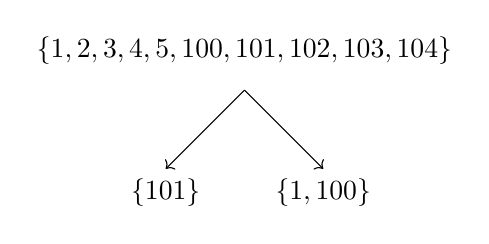
\begin{tikzpicture}
		\node (0,0) {$\{ 1, 2, 3, 4, 5, 100, 101, 102, 103, 104 
			\}$};
		\draw[->] (0,-.5) -- (-1,-1.5);
		\draw[->] (0,-.5) -- (1,-1.5);
		\node[below] at (-1,-1.5) {$\{ 101 \}$};
		\node[below] at (1,-1.5) {$\{ 1, 100 \}$};
	\end{tikzpicture}
	\caption{An example of a 10-digit set split into two disjoint 
		subsets with the same sum.}\label{pigeon}
\end{marginfigure}

\begin{example}
	Given ten distinct positive integers less than 107, there exist 
	two disjoint subsets with the same sum. As an illustration, 
	consider Figure \ref{pigeon}.
	
	\begin{proof}
		The largest sum possible would be $\sum_{i=97}^{106} i = 
		1015$. We consider the possible sums of our subsets to be 
		the boxes referred to by the Pigeonhole Principle, and so 
		we have 1016 boxes (the subset being the empty set 
		corresponds to the box with sum of 0). But for a set 
		containing 10 numbers, we have $2^{10} = 1024$ subsets. By 
		the pigeonhole principle, at least two of these subsets 
		have the same sum since $1024 > 1016$. If they are not 
		disjoint, remove their intersection and they will still 
		have the same sum.
	\end{proof}
\end{example}

\begin{marginfigure}[1in]
	\centering
	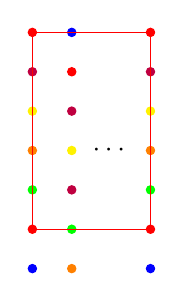
\begin{tikzpicture}
		\filldraw[blue] (0,0) circle (1.5pt);
		\filldraw[red] (0,.5) circle (1.5pt);
		\filldraw[green] (0,1) circle (1.5pt);
		\filldraw[orange] (0,1.5) circle (1.5pt);
		\filldraw[yellow] (0,2) circle (1.5pt);
		\filldraw[purple] (0,2.5) circle (1.5pt);
		\filldraw[red] (0,3) circle (1.5pt);
		
		\filldraw[orange] (.5,0) circle (1.5pt);
		\filldraw[green] (.5,.5) circle (1.5pt);
		\filldraw[purple] (.5,1) circle (1.5pt);
		\filldraw[yellow] (.5,1.5) circle (1.5pt);
		\filldraw[purple] (.5,2) circle (1.5pt);
		\filldraw[red] (.5,2.5) circle (1.5pt);
		\filldraw[blue] (.5,3) circle (1.5pt);
		
		\node at (1,1.5) {$\cdots$};
		
		\filldraw[blue] (1.5,0) circle (1.5pt);
		\filldraw[red] (1.5,.5) circle (1.5pt);
		\filldraw[green] (1.5,1) circle (1.5pt);
		\filldraw[orange] (1.5,1.5) circle (1.5pt);
		\filldraw[yellow] (1.5,2) circle (1.5pt);
		\filldraw[purple] (1.5,2.5) circle (1.5pt);
		\filldraw[red] (1.5,3) circle (1.5pt);
		
		\draw[red] (0,.5) -- (1.5,.5) -- (1.5,3) -- (0,3) -- (0,.5);
	\end{tikzpicture}
	\caption{Eventually the coloring of neighboring sets of seven 
	vertical vertices will have to repeat, yielding a rectangle 
	with monochromatic vertices.}\label{mono rect}
\end{marginfigure}

\begin{example}
	Consider $\reals^2$ restricted to integer coordinates. Show 
	there is no way to assign one of six colors to each vertex such 
	that there does not exist a rectangle whose vertices are 
	monochromatic.
	
	\begin{proof}
		I present a simplified version of the proof from class. 
		Consider a vertical column of seven vertices. Since there 
		are only 6 colors, any coloring of these seven vertices 
		will result in a repeated color. This repeated color is red 
		in the first vertical column of Figure \ref{mono rect}. 
		There are a finite number, let's say $k$, of ways to color 
		seven vertical vertices without repeating the coloring in 
		our first column. So if we pick $k+1$ neighboring columns 
		of seven vertices, then by the pigeonhole principle at 
		least two columns must share the same coloring. This will 
		yield a rectangle with monochromatic vertices, drawn in red 
		in Figure \ref{mono rect}.
	\end{proof}
\end{example}



































\appendix

\chapter{Solutions to Shoenfield's \emph{Mathematical Logic}}

\section{The Nature of Mathematical Logic}

No exercises.

%%%%%%%%%%%%%%%%%%%%%%%%%%%%%%%%%%%%%%%%%%%%%%%%%%%%%%%%%%%%%%%%%%
%%%%%%%%%%%%%%%%%%%%%%%%%%%%%%%%%%%%%%%%%%%%%%%%%%%%%%%%%%%%%%%%%%

\section{First-Order Theories}

\begin{exercise}
	An $n$-ary truth function $H$ is \df{definable in terms of} the 
	truth functions $H_1, \dots, H_k$ if $H$ has a definition
	\[
		H(\nms{a}) = ...\,,
	\]
	where the right-hand side is built up from $H_1, \dots, H_k, 
	a_1, \dots, a_n$, and commas and parentheses.
	\begin{enumerate}
		\item[a)] Let $H_{d,n}$ be the truth function defined by 
		setting $H_{d,n}(\nms{a}) = \bt{T}$ if and only if $a_i = 
		\bt{T}$ for at least one $i$, and let $H_{c,n}$ be the 
		truth function defined by setting
		\[
			H_{c,n}(\nms{a}) = \bt{T}
			\quad
			\text{if and only if}
			\quad 
			a_i = \bt{T} \text{ for all } i\,.
		\]
		Show that every truth function is definable in terms of 
		$\Hneg{}$ and certain of the $H_{d,n}$ and $H_{c,n}$.
		
		\item[b)] Show that every truth function is definable in 
		terms of $\Hneg{}$ and $\Hor{}$. [Use (a).]
		
		\item[c)] Show that every truth function is definable in 
		terms of $\Hneg{}$ and $\Hra{}$. [Use (b).]
		
		\item[d)] Show that every truth function is definable in 
		terms of $\Hneg{}$ and $\Hand{}$. [Use (b).]
		
		\item[e)] Show that $\Hneg{}$ is not definable in terms of 
		$\Hor{}$, $\Hra{}$, $\Hand{}$, and $\Hlra{}$.
	\end{enumerate}
\end{exercise}

%%%%%%%%%%%%%%%%%%%%%%%%%%%%%%%%%%%%%%%%%%%%%%%%%%%%%%%%%%%%%%%%%%

\begin{proof}
	\begin{enumerate}
		\item[a)] We first consider the case where $H = \bt{F}$ for 
		every valuation. Then we define $H$ as
		\[
			H(\nms{a}) = H_{d,n} \left( H_{c,2}(a_1,\Hneg{}(a_1)), 
			\dots, H_{c,2}(a_n,\Hneg{}(a_n)) \right)\,,
		\]
		which always evaluates to \bt{F}.
		
		Now suppose $H = \bt{T}$ for $m$ $n$-tuples $(\nms{a})_i$ 
		for $i = 1, \dots, m$. Then for those $m$ $n$-tuples define 
		$H_{c,n}(i)$ as replacing all $a_j = \bt{F}$ in 
		$(\nms{a})_i$ with $\Hneg{}(a_j)$. Then we define $H$ as
		\[
			H(\nms{a}) = (H_{c,n}(1), \dots, H_{c,n}(m))\,,
		\]
		which always evaluates to \bt{T}.
		
		\item[b)] We show that $H_{d,n}$ is definable in terms of 
		$\Hor$, which in turn constitutes a proof due to (a). We 
		define $H_{d,n}$ as
		\[
			H_{d,n} = 
			\Hor{}(a_1, \dots, \Hor{}(a_{n-2},\Hor{}(a_{n-1}, 
			\Hor{}(a_n))))\,.
		\]
		
		\item[c)] We know that $\Hra{}(a,b) = 
		\Hor{}(\Hneg{}(a),b)$.
	\end{enumerate}
\end{proof}

%%%%%%%%%%%%%%%%%%%%%%%%%%%%%%%%%%%%%%%%%%%%%%%%%%%%%%%%%%%%%%%%%%

\begin{exercise}
	$ $
	\begin{enumerate}
		\item[a)] Let $H_d$ be the truth function defined by
		\[
			H_d(a,b) = \bt{T} \text{ if and only if } a = b = 
			\bt{T}\,.
		\]
		Show that every truth function is definable in terms of 
		$H_d$. [Use 1(b).]
		
		\item[b)] Let $H_a$ be the truth function defined by
		\[
			H_a(a,b) = \bt{F} \text{ if and only if } a = b = 
			\bt{T}\,.
		\]
		Show that every truth function is definable in terms of 
		$H_a$.
		
		\item[c)] A truth function $H$ is \df{singulary} if there 
		is a truth function $H'$ and an $i$ such that $H(\nms{a}) = 
		H'(a_i)$ for all $\nms{a}$. Show that if $H$ is singulary, 
		then every truth function definable in terms of $H$ is 
		singulary.
		
		\item[d)] Show that if $H$ is a binary truth function such 
		that every truth function is definable in terms of $H$, 
		then $H$ is $H_d$ or $H_a$. [Show that $H(\bt{T}, \bt{T}) = 
		\bt{F}$ and $H(\bt{F},\bt{F}) = \bt{T}$, and use (c).]
	\end{enumerate}
\end{exercise}

%%%%%%%%%%%%%%%%%%%%%%%%%%%%%%%%%%%%%%%%%%%%%%%%%%%%%%%%%%%%%%%%%%

\begin{proof}
	asdf
\end{proof}

%%%%%%%%%%%%%%%%%%%%%%%%%%%%%%%%%%%%%%%%%%%%%%%%%%%%%%%%%%%%%%%%%%

\begin{exercise}
	Show that if $\bt{u}\bt{v}$ and $\bt{v}\bt{v}'$ are 
	designators, then either \bt{v} or $\bt{v}'$ is the empty 
	expression.
\end{exercise}

%%%%%%%%%%%%%%%%%%%%%%%%%%%%%%%%%%%%%%%%%%%%%%%%%%%%%%%%%%%%%%%%%%

\begin{proof}
	Suppose $\bt{u}\bt{v}$ and $\bt{v}\bt{v}'$ are designators. We 
	use induction on the length of $\bt{u}\bt{v}$. If 
	$\bt{u}\bt{v}$ is a variable, then either \bt{u} or \bt{v} are 
	empty (since variables have length 1). If \bt{v} is empty, we 
	are done, so suppose \bt{u} is empty and \bt{v} is a variable. 
	But then $\bt{v}\bt{v}'$ can only be a designator if $\bt{v}'$ 
	is empty because the only way to obtain a new designator from a 
	variable is to add either a function symbol or predicate symbol 
	to the left of the variable.
	
	If $\bt{u}\bt{v}$ is an arbitrary term or formula, it is still 
	the case that 
\end{proof}

%%%%%%%%%%%%%%%%%%%%%%%%%%%%%%%%%%%%%%%%%%%%%%%%%%%%%%%%%%%%%%%%%%

\begin{exercise}
	Show that the result of replacing \bt{a} by \bt{x} in a term is 
	a term, and that the result of replacing \bt{a} by \bt{x} in a 
	formula is a formula.
\end{exercise}

%%%%%%%%%%%%%%%%%%%%%%%%%%%%%%%%%%%%%%%%%%%%%%%%%%%%%%%%%%%%%%%%%%

\begin{proof}
	asdf
\end{proof}

%%%%%%%%%%%%%%%%%%%%%%%%%%%%%%%%%%%%%%%%%%%%%%%%%%%%%%%%%%%%%%%%%%

\begin{exercise}
	Let $T$ be the theory with no nonlogical symbols and no 
	nonlogical axioms.
\end{exercise}







































\chapter{Solutions to D\&F's \emph{Abstract Algebra}}

\section*{Preliminaries}

\subsection{Basics}

In Exercises 1 to 4 let $\mc{A}$ be the set of $2 \times 2$ matrices with real number entries. Recall that matrix multiplication is defined by
\[
	\begin{pmatrix}
		a & b \\
		c & d
	\end{pmatrix}
	\begin{pmatrix}
		p & q \\
		r & s
	\end{pmatrix}
	=
	\begin{pmatrix}
		ap + br & aq + bs \\
		cp + dr & cq + ds
	\end{pmatrix}\,.
\]
Let
\[
	M = 
	\begin{pmatrix}
		1 & 1 \\
		0 & 1
	\end{pmatrix}
\]
and let
\[
	\mc{B} = \{ X \in \mc{A} \mid MX = XM \}\,.
\]

\begin{exercise}
	Determine which of the following elements of $\mc{A}$ lie in $\mc{B}$:
	\[
		\begin{pmatrix}
			1 & 1 \\
			0 & 1
		\end{pmatrix},
		\quad
		\begin{pmatrix}
			1 & 1 \\
			1 & 1
		\end{pmatrix},
		\quad
		\begin{pmatrix}
			0 & 0 \\
			0 & 0
		\end{pmatrix},
		\quad
		\begin{pmatrix}
			1 & 1 \\
			1 & 0
		\end{pmatrix},
		\quad
		\begin{pmatrix}
			1 & 0 \\
			0 & 1
		\end{pmatrix},
		\quad
		\begin{pmatrix}
			0 & 1 \\
			1 & 0
		\end{pmatrix}\,.
	\]
\end{exercise}

\begin{proof}[Solution]
	We have
	\begin{align*}
		\begin{pmatrix}
			1 & 1 \\
			0 & 1
		\end{pmatrix}
		\begin{pmatrix}
			1 & 1 \\
			0 & 1
		\end{pmatrix}
		&=
		\begin{pmatrix}
			1 & 1 \\
			0 & 1
		\end{pmatrix}
		\begin{pmatrix}
			1 & 1 \\
			0 & 1
		\end{pmatrix}\,,
		\text{ so }	
		\begin{pmatrix}
			1 & 1 \\
			0 & 1
		\end{pmatrix}
		\in \mc{B}\,;
		\\
		\begin{pmatrix}
			1 & 1 \\
			0 & 1
		\end{pmatrix}
		\begin{pmatrix}
			1 & 1 \\
			1 & 1
		\end{pmatrix}
		&=
		\begin{pmatrix}
			2 & 2 \\
			1 & 1
		\end{pmatrix}\,,
		\text{ and }
		\begin{pmatrix}
			1 & 1 \\
			1 & 1
		\end{pmatrix}
		\begin{pmatrix}
			1 & 1 \\
			0 & 1
		\end{pmatrix}
		=
		\begin{pmatrix}
			1 & 2 \\
			1 & 2
		\end{pmatrix}\,,
		\\
		&\text{ so }
		\begin{pmatrix}
			1 & 1 \\
			1 & 1
		\end{pmatrix}
		\notin \mc{B}\,;
		\\
		\begin{pmatrix}
			1 & 1 \\
			0 & 1
		\end{pmatrix}
		\begin{pmatrix}
			0 & 0 \\
			0 & 0
		\end{pmatrix}
		&=
		\begin{pmatrix}
			0 & 0 \\
			0 & 0
		\end{pmatrix}
		\begin{pmatrix}
			1 & 1 \\
			0 & 1
		\end{pmatrix}\,,
		\text{ so }
		\begin{pmatrix}
			0 & 0 \\
			0 & 0
		\end{pmatrix}
		\in \mc{B}\,;
		\\
		\begin{pmatrix}
			1 & 1 \\
			0 & 1
		\end{pmatrix}
		\begin{pmatrix}
			1 & 1 \\
			1 & 0
		\end{pmatrix}
		&=
		\begin{pmatrix}
			2 & 1 \\
			1 & 0
		\end{pmatrix}\,,
		\text{ and }
		\begin{pmatrix}
			1 & 1 \\
			1 & 0
		\end{pmatrix}
		\begin{pmatrix}
			1 & 1 \\
			0 & 1
		\end{pmatrix}
		=
		\begin{pmatrix}
			1 & 2 \\
			1 & 1
		\end{pmatrix}\,,
		\\
		&\text{ so }
		\begin{pmatrix}
			1 & 1 \\
			1 & 0
		\end{pmatrix}
		\notin \mc{B}\,;
		\\
		\begin{pmatrix}
			1 & 1 \\
			0 & 1
		\end{pmatrix}
		\begin{pmatrix}
			1 & 0 \\
			0 & 1
		\end{pmatrix}
		&=
		\begin{pmatrix}
			1 & 0 \\
			0 & 1
		\end{pmatrix}
		\begin{pmatrix}
			1 & 1 \\
			0 & 1
		\end{pmatrix}\,,
		\text{ so }	
		\begin{pmatrix}
			1 & 0 \\
			0 & 1
		\end{pmatrix}
		\in \mc{B}\,;
		\\
		\begin{pmatrix}
			1 & 1 \\
			0 & 1
		\end{pmatrix}
		\begin{pmatrix}
			0 & 1 \\
			1 & 0
		\end{pmatrix}
		&=
		\begin{pmatrix}
			1 & 1 \\
			1 & 0
		\end{pmatrix}\,,
		\text{ and }
		\begin{pmatrix}
			0 & 1 \\
			1 & 0
		\end{pmatrix}
		\begin{pmatrix}
			1 & 1 \\
			0 & 1
		\end{pmatrix}
		=
		\begin{pmatrix}
			0 & 1 \\
			1 & 1
		\end{pmatrix}\,,
		\\
		&\text{ so }
		\begin{pmatrix}
			0 & 1 \\
			1 & 0
		\end{pmatrix}
		\notin \mc{B}\,;
	\end{align*}
\end{proof}

%%%%%%%%%%%%%%%%%%%%%%%%%%%%%%%%%%%%%%%%%%%%%%%%%%%%%%%%%%%%%%%%%%

\begin{exercise}
	Prove that if $P, Q \in \mc{B}$, then $P + Q \in \mc{B}$ (where + denotes the usual sum of two matrices).
\end{exercise}

\begin{proof}
	We have
	\[
		M(P + Q) = MP + MQ = PM + QM = (P + Q)M\,.
	\]
\end{proof}

%%%%%%%%%%%%%%%%%%%%%%%%%%%%%%%%%%%%%%%%%%%%%%%%%%%%%%%%%%%%%%%%%%

\begin{exercise}
	Prove that if $P, Q \in \mc{B}$, then $P \cdot Q \in \mc{B}$ (where $\cdot$ denotes the usual product of two matrices).
\end{exercise}

\begin{proof}
	We have
	\[
		M(PQ) = (MP)Q = (PM)Q = P(MQ) = P(QM) = (PQ)M\,.
	\]
\end{proof}

%%%%%%%%%%%%%%%%%%%%%%%%%%%%%%%%%%%%%%%%%%%%%%%%%%%%%%%%%%%%%%%%%%

\begin{exercise}
	Find conditions on $p, q, r, s$ which determine precisely when
	$\begin{pmatrix}
		p & q \\
		r & s
	\end{pmatrix}
	\in \mc{B}$.
\end{exercise}

\begin{proof}[Solution]
	We have
	\[
		\begin{pmatrix}
			1 & 1 \\
			0 & 1
		\end{pmatrix}
		\begin{pmatrix}
			p & q \\
			r & s
		\end{pmatrix}
		=
		\begin{pmatrix}
			p + r & q + s \\
			r & s
		\end{pmatrix}\,,
	\]
	and
	\[
		\begin{pmatrix}
			p & q \\
			r & s
		\end{pmatrix}
		\begin{pmatrix}
			1 & 1 \\
			0 & 1
		\end{pmatrix}
		=
		\begin{pmatrix}
			p & p + q \\
			r & r + s
		\end{pmatrix}\,.
	\]
	Setting these resultant matrices equal to each other yields the required condition: $r = 0$ and $p = s$.
\end{proof}

%%%%%%%%%%%%%%%%%%%%%%%%%%%%%%%%%%%%%%%%%%%%%%%%%%%%%%%%%%%%%%%%%%

\begin{exercise}
	Determine whether the following functions $f$ are well defined:
	\begin{enumerate}
		\item[(a)] $f : \rationals \to \integers$ defined by $f(a/b)
			= a$.
		\item[(b)] $f : \rationals \to \rationals$ defined by
			$f(a/b) = a^2/b^2$.
	\end{enumerate}
\end{exercise}

\begin{proof}[Solution]
	\begin{enumerate}
		\item[(a)] This function $f$ is not well defined for the
			following two reasons: $f(1/2) \neq f(2/4)$ and $f(-1/2) \neq f(1/-2)$.
			
		\item[(b)] This function $f$ is well defined, since any
			negatives will be squared away and equivalent ways of writing a fraction give the same result: $f(na/nb) = n^2a^2/n^2b^2 = a^2/b^2 = f(a/b)$.
	\end{enumerate}
\end{proof}

%%%%%%%%%%%%%%%%%%%%%%%%%%%%%%%%%%%%%%%%%%%%%%%%%%%%%%%%%%%%%%%%%%

\begin{exercise}
	Determine whether the function $f : \rplus \to \integers$ defined by mapping a real number $r$ to the first digit to the right of the decimal point in a decimal expansion of $r$ is well defined.
\end{exercise}

\begin{proof}[Solution]
	This function $f$ is not well defined since $f(.\bar{9}) = 9$ 
	and $f(1) = 0$ even though $.\bar{9} = 1$.
\end{proof}

%%%%%%%%%%%%%%%%%%%%%%%%%%%%%%%%%%%%%%%%%%%%%%%%%%%%%%%%%%%%%%%%%%

\begin{exercise}
	Let $f : A \to B$ be a surjective map of sets. Prove that the relation
	\[
		a \sim b \text{ if and only if } f(a) = f(b)
	\]
	is an equivalence relation whose equivalence classes are the fibers of $f$.
\end{exercise}

\begin{proof}
	We first prove $\sim$ is reflexive. Since $f$ is well defined, $f(a) = f(a)$. Next we prove $\sim$ is symmetric. If $f(a) = f(b)$, then $f(b) = f(a)$. Finally, we show $\sim$ is transitive. If $f(a) = f(b)$ and $f(b) = f(c)$, then $f(a) = f(c)$.
	
	We now need to show that the equivalence classes of $\sim$ are the fibers of $f$. $a \sim b$ means $f(a) = f(b)$. This means that $a$ and $b$ map to the same element of $B$; that is, they belong to the same fiber of $f$.
\end{proof}

%%%%%%%%%%%%%%%%%%%%%%%%%%%%%%%%%%%%%%%%%%%%%%%%%%%%%%%%%%%%%%%%%%
%%%%%%%%%%%%%%%%%%%%%%%%%%%%%%%%%%%%%%%%%%%%%%%%%%%%%%%%%%%%%%%%%%

\subsection{Properties of the Integers}

\begin{exercise}
	For each of the following pairs of integers $a$ and $b$, determine their greatest common divisor, their least common multiple, and write their greatest common divisor in the form $ax + by$ for some integers $x$ and $y$.
	\begin{enumerate}
		\item[(a)] $a = 20$, $b = 13$.
		\item[(b)] $a = 69$, $b = 372$.
		\item[(c)] $a = 792$, $b = 275$.
		\item[(d)] $a = 11391$, $b = 5673$.
		\item[(e)] $a = 1761$, $b = 1567$.
		\item[(f)] $a = 507885$, $b = 60808$.
	\end{enumerate}
\end{exercise}

\begin{proof}[Solution]
	\begin{enumerate}
		\item[(a)] We first find the g.c.d.:
			\begin{align*}
				20 &= (1)(13) + 7 \\
				13 &= (1)(7) + 6 \\
				7 &= (1)(6) + 1 \\
				6 &= (6)(1)\,.
			\end{align*}
			So $\gcd(20,13) = 1$.
			
			We now find the l.c.m. We have $\gcd(a,b)\lcm(a,b) = ab$, and so
			\[
				\lcm(20,13) = \frac{20(13)}{\gcd(20,13)} = 260\,.
			\]
			
			We now write the g.c.d. in the form $ax + by$:
			\begin{align*}
				1 &= 7 - (1)(6) \\
					&= 7 - (1)[13 - (1)(7)] \\
					&= (2)7 - (13)1 \\
					&= (2)[20 - (1)13] - 13(1) \\
					&= (2)20 - (3)13
			\end{align*}
		\item[(b)] We first find the g.c.d.:
			\begin{align*}
				69 &= (0)(372) + 69 \\
				372 &= (5)(69) + 27 \\
				69 &= (2)(27) + 15 \\
				27 &= (1)(15) + 12 \\
				15 &= (1)(12) + 3 \\
				12 &= (4)(3)\,.
			\end{align*}
			So $\gcd(69,372) = 3$.
			
			We now find the l.c.m.:
			\[
				\lcm(69,372) = \frac{69(372)}{3} = 8556\,.
			\]
			
			We now write the g.c.d. in the form $ax + by$:
			\begin{align*}
				3 &= 15 - (1)(12) \\
					&= 15 - [27 - 15] \\
					&= (2)15 - 27 \\
					&= (2)[69 - 2(27)] - 27 \\
					&= (2)69 - 5(27) \\
					&= (2)69 - 5[372 - (5)69] \\
					&= (27)69 - (5)372\,.
			\end{align*}
		\item[(c)] We first find the g.c.d.:
			\begin{align*}
				792 &= 2(275) + 242 \\
				275 &= 1(242) + 33 \\
				242 &= 7(33) + 11 \\
				33 &= 3(11)\,.
			\end{align*}
			So $\gcd(792,275) = 11$.
			
			We now find the l.c.m.:
			\[
				\lcm(792,275) = \frac{792(275)}{11} = 19800\,.
			\]
			
			We now write the g.c.d. in the form $ax + by$:
			\begin{align*}
				11 &= 242 - 7(33) \\
					&= 242 - 7[275 - 242] \\
					&= (8)242 - (7)275 \\
					&= 8[792 - (2)275] - (7)275 \\
					&= (8)792 - (23)275\,.
			\end{align*}
		\item[(d)] We first find the g.c.d.:
			\begin{align*}
				11391 &= 2(5673) + 45 \\
				5673 &= 126(45) + 3 \\
				45 &= 15(3)\,.
			\end{align*}
			So $\gcd(11391,5673) = 3$.
			
			We now find the l.c.m.:
			\[
				\lcm(11391,5673) = \frac{11391(5673)}{3} = 21540381\,.
			\]
			
			We now write the g.c.d. in the form $ax + by$:
			\begin{align*}
				3 &= 5673 - 126(45) \\
					&= 5673 - 126[11391 - 2(5673)] \\
					&= (253)5673 - (126)11391\,.
			\end{align*}
		\item[(e)] We first find the g.c.d.:
			\begin{align*}
				1761 &= (1)1567 + 194 \\
				1567 &= (8)194 + 15 \\
				194 &= (12)15 + 14 \\
				15 &= (1)14 + 1 \\
				14 &= (14)1\,.
			\end{align*}
			So $\gcd(1761,1567) = 1$.
			
			We now find the l.c.m.:
			\[
				\lcm(1761,1567) = \frac{1761(1567)}{1} = 2759487\,.
			\]
			
			We now write the g.c.d. in the form $ax + by$:
			\begin{align*}
				1 &= 15 - 14 \\
					&= 15 - [194 - (12)15] \\
					&= (13)15 - 194 \\
					&= (13)[1567 - (8)194] - 194 \\
					&= (13)1567 - (105)194 \\
					&= (13)1567 - (105)[1761 - 1567] \\
					&= (118)1567 - (105)1761\,.
			\end{align*}
		\item[(f)] We first find the g.c.d.:
			\begin{align*}
				507885 &= (8)60808 + 21421 \\
				60808 &= (2)21421 + 17966 \\
				21421 &= (1)17966 + 3455 \\
				17966 &= (5)3455 + 691 \\
				3455 &= (5)691\,.
			\end{align*}
			So $\gcd(507885,60808) = 691$.
			
			We now find the l.c.m.:
			\[
				\lcm(507885,60808) = \frac{507885(60808)}{691} = 44693880\,.
			\]
			
			We now write the g.c.d. in the form $ax + by$:
			\begin{align*}
				691 &= 17966 - (5)3455 \\
					&= 17966 - (5)[21421 - 17966] \\
					&= (6)17966 - (5)21421 \\
					&= (6)[60808 - (2)21421] - (5)21421 \\
					&= (6)60808 - (17)21421 \\
					&= (6)60808 - (17)[507885 - (8)60808] \\
					&= (142)60808 - (17)507885\,.
			\end{align*}
	\end{enumerate}
\end{proof}

%%%%%%%%%%%%%%%%%%%%%%%%%%%%%%%%%%%%%%%%%%%%%%%%%%%%%%%%%%%%%%%%%%

\begin{exercise}
	Prove that if the integer $k$ divides the integers $a$ and $b$ then $k$ divides $as + bt$ for every pair of integers $s$ and $t$.
\end{exercise}

\begin{proof}
	Suppose $k \mid a$ and $k \mid b$. Then $a = km$ and $b = nk$ for some integers $m$ and $n$. So $as + bt = mks + nkt = k(ms + nt)$, and therefore $k \mid (as + bt)$.
\end{proof}

%%%%%%%%%%%%%%%%%%%%%%%%%%%%%%%%%%%%%%%%%%%%%%%%%%%%%%%%%%%%%%%%%%

\begin{exercise}
	Prove that if $n$ is composite then there are integers $a$ and $b$ such that $n$ divides $ab$ but $n$ does not divide either $a$ or $b$.
\end{exercise}

\begin{proof}
	Suppose $n$ is composite. Then $n = ab$ for some $a$ and $b$ with $|a| < n$ and $|b| < n$. Since $n = ab$, $n \mid ab$, but $n \nmid a$ and $n \nmid b$ since $|a| < n$ and $|b| < n$.
\end{proof}

%%%%%%%%%%%%%%%%%%%%%%%%%%%%%%%%%%%%%%%%%%%%%%%%%%%%%%%%%%%%%%%%%%

\begin{exercise}
	Let $a,b$ and $N$ be fixed integers with $a$ and $b$ nonzero and let $d = \gcd(a,b)$ be the greatest common divisor of $a$ and $b$. Suppose $x_0$ and $y_0$ are particular solutions to $ax + by = N$ (i.e., $ax_0 + by_0 = N$). Prove for any integer $t$ that the integers
	\[
		x = x_0 + \frac{b}{d}t
		\quad
		\text{and}
		\quad
		y = y_0 - \frac{a}{d}t
	\]
	are also solutions to $ax + by = N$ (this is in fact the general solution).
\end{exercise}

\begin{proof}
	Suppose $ax + by = N$ has the particular solutions $x_0$ and $y_0$; that is, suppose $ax_0 + by_0 = N$. Let $t$ be arbitrary. Then
	\[
		a \left( x_0 + \frac{b}{d}t \right) +
		b \left( y_0 - \frac{a}{d}t \right) 
			= ax_0 + \frac{ab}{d}t + by_0 - \frac{ab}{d}t
			= N\,.
	\]
\end{proof}

%%%%%%%%%%%%%%%%%%%%%%%%%%%%%%%%%%%%%%%%%%%%%%%%%%%%%%%%%%%%%%%%%%

\begin{exercise}
	Determine the value $\varphi(n)$ for each integer $n \leq 30$ where $\varphi$ denotes the Euler $\varphi$-function.
\end{exercise}

\begin{proof}[Solution]
	We have $\varphi(1) = 1$, $\varphi(2) = 1$, $\varphi(3) = 2$, $\varphi(4) = 2$, $\varphi(5) = 4$, $\varphi(6) = 2$, $\varphi(7) = 6$, $\varphi(8) = \varphi(2^3) = 2^{3-1}(2-1) = 4$, $\varphi(9) = \varphi(3^2) = 3(3-1) = 6$, $\varphi(10) = \varphi(2)\varphi(5) = 4$, $\varphi(11) = 10$, $\varphi(12) = \varphi(3)\varphi(4) = 2(2) = 4$, $\varphi(13) = 12$, $\varphi(14) = \varphi(2)\varphi(7) = 6$, $\varphi(15) = \varphi(3)\varphi(5) = 2(4) = 8$, $\varphi(16) = \varphi(2^4) = 2^3(2-1) = 8$, $\varphi(17) = 16$, $\varphi(18) = \varphi(2)\varphi(9) = 6$, $\varphi(19) = 18$, $\varphi(20) = \varphi(4)\varphi(5) = 8$, $\varphi(21) = \varphi(3)\varphi(7) = 12$, $\varphi(22) = \varphi(2)\varphi(11) = 10$, $\varphi(23) = 22$, $\varphi(24) = \varphi(3)\varphi(8) = 8$, $\varphi(25) = \varphi(5^2) = 5(4) = 20$, $\varphi(26) = \varphi(2)\varphi(13) = 12$, $\varphi(27) = \varphi(3^3) = 3^2(2) = 18$, $\varphi(28) = \varphi(4)\varphi(7) = 12$, $\varphi(29) = 28$, $\varphi(30) = \varphi(3)\varphi(10) = 8$.
\end{proof}

%%%%%%%%%%%%%%%%%%%%%%%%%%%%%%%%%%%%%%%%%%%%%%%%%%%%%%%%%%%%%%%%%%

\begin{exercise}
	Prove the Well Ordering Property of $\integers$ by induction and prove the minimal element is unique.
\end{exercise}

\begin{proof}
	Let $A$ be an arbitrary nonempty subset of $\zplus$.
	
	Base Case: $A$ has a single element. Then this element is the minimal element of $A$, for $m \leq m$. Moreover, being the only element, it is unique.
	
	Inductive Step: Now suppose $A$ has $n$ elements, and the theorem holds for any set of $n$ or fewer elements. We show the theorem holds for a set of $n + 1$ elements. If new element is smaller than existing minimal element, it is the minimal element. Otherwise, the existing minimal element remains the minimal element.
\end{proof}

%%%%%%%%%%%%%%%%%%%%%%%%%%%%%%%%%%%%%%%%%%%%%%%%%%%%%%%%%%%%%%%%%%

\begin{exercise}
	If $p$ is a prime prove that there do not exist nonzero integers $a$ and $b$ such that $a^2 = pb^2$ (i.e., $\sqrt{p}$ is not a rational number).
\end{exercise}

\begin{proof}
	By way of contradiction, suppose $p$ is prime and there exists 
	$a,b$ such that $a^2 = pb^2$; that is, $\sqrt{p} = 
	\frac{a}{b}$. Assume $\gcd(a,b) = 1$; that is, suppose 
	$\sqrt{p}$ is written in its most reduced form. Then $p \mid 
	a^2$, and so $p \mid a$. That is, $a = pc$ for some integer 
	$c$. Then $a^2 = p^2c^2 = pb^2$. And so, $pc^2 = b^2$, and we 
	see that $p \mid b^2$ and so $p \mid b$. Since $p \mid a$ and 
	$p \mid b$, then $p \mid ab$, contradicting the fact that 
	$\gcd(a,b) = 1$.
\end{proof}

%%%%%%%%%%%%%%%%%%%%%%%%%%%%%%%%%%%%%%%%%%%%%%%%%%%%%%%%%%%%%%%%%%

\begin{exercise}
	Let $p$ be a prime, $n \in \zplus$. Find a formula for the largest power of $p$ which divides $n! = n(n-1)(n-2) \cdots 2 \cdot 1$ (it involves the greatest integer function).
\end{exercise}

\begin{proof}[Solution]
	There are $\left\lfloor \frac{n}{p^k} \right\rfloor$ multiples 
	of $p^k$ in the list $1, 2, \dots, n$; that is, $p^k$ divides 
	$\left\lfloor \frac{n}{p^k} \right\rfloor$ numbers less than or 
	equal to $n$. Thus, $\sum_k \left\lfloor \frac{n}{p^k} 
	\right\rfloor$ accounts for the highest order of $p$ which 
	divides $n!$.
\end{proof}

%%%%%%%%%%%%%%%%%%%%%%%%%%%%%%%%%%%%%%%%%%%%%%%%%%%%%%%%%%%%%%%%%%

\begin{exercise}
	Write a computer program to determine the greatest common divisor $\gcd(a,b)$ of two integers $a$ and $b$ and to express $\gcd(a,b)$ in the form $ax + by$ for some integers $x$ and $y$.
\end{exercise}

\begin{proof}[Solution]
	\lstinputlisting[language=python]{Solutions/gcd.py}
\end{proof}

%%%%%%%%%%%%%%%%%%%%%%%%%%%%%%%%%%%%%%%%%%%%%%%%%%%%%%%%%%%%%%%%%%

\begin{exercise}
	Prove for any given positive integer $N$ there exist only finitely many integers $n$ with $\varphi(n) = N$ where $\varphi$ denotes Euler's $\varphi$-function. Conclude in particular that $\varphi(n)$ tends to infinity as $n$ tends to infinity.
\end{exercise}

\begin{proof}
	Let $N \in \zplus$ be arbitrary. For any $n = p_1^{\alpha_1} 
	\cdots p_s^{\alpha_s}$ such that $\varphi(n)  = p_1^{\alpha_1 - 
	1}(p_1 - 1) \cdots p_s^{\alpha_s - 1}(p_s - 1) = N$, it is 
	clear from this formula that for any prime factor $p_i$ of $n$, 
	we have $\varphi(p_i) = p_i - 1 \mid N$. Thus $p_i - 1 \leq N$, 
	or $p_i \leq N + 1$.
	
	Therefore, let $p_1, \cdots, p_t$ be the primes which are less 
	than or equal to $N + 1$. All $n$ such that $\varphi(n) = N$ 
	thus have prime factorizations of the form $p_1^{\alpha_1} 
	\cdots p_t^{\alpha_t}$. Moreover, for $1 \leq i \leq t$, we 
	have $p_i^{\alpha_i - 1} \mid N$. Let $k_i$ be the largest 
	integer such that $p_i^{k_i} \mid N$. Obviously, $\alpha_i \leq 
	k_i + 1$, and so there are at most $\prod_i (k_i + 1)$ integers 
	$n$ such that $\varphi(n) = N$.
\end{proof}

%%%%%%%%%%%%%%%%%%%%%%%%%%%%%%%%%%%%%%%%%%%%%%%%%%%%%%%%%%%%%%%%%%

\begin{exercise}
	Prove that if $d$ divides $n$ then $\varphi(d)$ divides $\varphi(n)$ where $\varphi$ denotes Euler's $\varphi$-function.
\end{exercise}

\begin{proof}
	Suppose $d \mid n$, and let the prime factorizations of $n$ and 
	$d$ be $n = p_1^{\alpha_1} p_2^{\alpha_2} \cdots 
	p_s^{\alpha_s}$ and $d = p_1^{\beta_1} p_2^{\beta_2} \cdots 
	p_s^{\beta_s}p_{s+1}^{\beta_{s+1}} \cdots p_t^{\beta_t}$, where 
	$\beta_i \geq \alpha_i$ for $1 \leq i \leq s$.
	
	We have
	\[
		\varphi(n) = p_1^{\alpha_1 - 1}(p_1 - 1) \cdots 
		p_s^{\alpha_s - 1}(p_s - 1)\,,
	\]
	and therefore
	\begin{align*}
		\varphi(d) &= p_1^{\beta_1 - 1}(p_1 - 1) \cdots p_s^{\beta_s
			- 1}(p_s - 1) p_{s+1}^{\beta_{s+1} - 1}(p_{s+1} - 1) 
			\cdots p_t^{\beta_t - 1}(p_t - 1) \\
		&= p_1^{\alpha_1 - 1} p_1^{\gamma_1} (p_1 - 1) \cdots 
			p_s^{\alpha_s - 1} p_1^{\gamma_s} (p_s - 1)
			p_{s+1}^{\beta_{s+1} - 1}(p_{s+1} - 1) \cdots 
			p_t^{\beta_t - 1}(p_t - 1) \\
		&= \varphi(n) p_1^{\gamma_1} \cdots p_s^{\gamma_s} 
			p_{s+1}^{\beta_{s+1} - 1}(p_{s+1} - 1) \cdots 
			p_t^{\beta_t - 1}(p_t - 1)\,.
	\end{align*}	
	And so we have that $\varphi(n) \mid \varphi(d)$.
\end{proof}

%%%%%%%%%%%%%%%%%%%%%%%%%%%%%%%%%%%%%%%%%%%%%%%%%%%%%%%%%%%%%%%%%%
%%%%%%%%%%%%%%%%%%%%%%%%%%%%%%%%%%%%%%%%%%%%%%%%%%%%%%%%%%%%%%%%%%

\subsection{$\integers/n\integers$: The Integers Modulo $n$}

\begin{exercise}
	Write down explicitly all the elements in the residue classes of $\integers/18\integers$.
\end{exercise}

%%%%%%%%%%%%%%%%%%%%%%%%%%%%%%%%%%%%%%%%%%%%%%%%%%%%%%%%%%%%%%%%%%

\begin{exercise}
	Prove that the distinct equivalence classes in $\integers/n\integers$ are precisely $\bar{0}, \bar{1}, \bar{2}, \dots, \overline{n-1}$ (use the Division Algorithm).
\end{exercise}

%%%%%%%%%%%%%%%%%%%%%%%%%%%%%%%%%%%%%%%%%%%%%%%%%%%%%%%%%%%%%%%%%%

\begin{exercise}
	Prove that if $a = a_n 10^n + a_{n-1} 10^{n-1} + \cdots + a_1 10 + a_0$ is any positive integer then $a \equiv_9 a_n + a_{n-1} + \cdots a_1 + a_0$ (note that this is the usual arithmetic rule that the remainder after division by 9 is the same as the sum of the decimal digits mod 9--in particular an integer is divisible by 9 if and only if the sum of its digits is divisible by 9) [note that $10 \equiv_9 1$].
\end{exercise}

%%%%%%%%%%%%%%%%%%%%%%%%%%%%%%%%%%%%%%%%%%%%%%%%%%%%%%%%%%%%%%%%%%

\begin{exercise}
	Compute the remainder when $37^{100}$ is divided by 29.
\end{exercise}

%%%%%%%%%%%%%%%%%%%%%%%%%%%%%%%%%%%%%%%%%%%%%%%%%%%%%%%%%%%%%%%%%%

\begin{exercise}
	Compute the last two digits of $9^{1500}$.
\end{exercise}

%%%%%%%%%%%%%%%%%%%%%%%%%%%%%%%%%%%%%%%%%%%%%%%%%%%%%%%%%%%%%%%%%%

\begin{exercise}
	Prove that the squares of the elements in $\integers/4\integers$ are just $\bar{0}$ and $\bar{1}$.
\end{exercise}

%%%%%%%%%%%%%%%%%%%%%%%%%%%%%%%%%%%%%%%%%%%%%%%%%%%%%%%%%%%%%%%%%%

\begin{exercise}
	Prove for any integers $a$ and $b$ that $a^2 + b^2$ never leaves a remainder of 3 when divided by 4 (use the previous exercise).
\end{exercise}

%%%%%%%%%%%%%%%%%%%%%%%%%%%%%%%%%%%%%%%%%%%%%%%%%%%%%%%%%%%%%%%%%%

\begin{exercise}
	Prove that the equation $a^2 + b^2 = 3c^2$ has no solutions in nonzero integers $a$, $b$, and $c$. [Consider the equation mod 4 as in the previous two exercises and show that $a$, $b$, and $c$ would all have to be divisible by 2. Then each of $a^2$, $b^2$, and $c^2$ has a factor of 4 and by dividing through by 4 show that there would be a smaller set of solutions to the original equation. Iterate to reach a contradiction.]
\end{exercise}

%%%%%%%%%%%%%%%%%%%%%%%%%%%%%%%%%%%%%%%%%%%%%%%%%%%%%%%%%%%%%%%%%%

\begin{exercise}
	Prove that the square of any odd integer always leaves a remainder of 1 when divided by 8.
\end{exercise}

%%%%%%%%%%%%%%%%%%%%%%%%%%%%%%%%%%%%%%%%%%%%%%%%%%%%%%%%%%%%%%%%%%

\begin{exercise}
	Prove that the number of elements of $(\integers/n\integers)^\times$ is $\varphi(n)$ where $\varphi$ denotes the Euler $\varphi$-function.
\end{exercise}

%%%%%%%%%%%%%%%%%%%%%%%%%%%%%%%%%%%%%%%%%%%%%%%%%%%%%%%%%%%%%%%%%%

\begin{exercise}
	Prove that if $\bar{a}, \bar{b} \in (\integers/n\integers)^\times$, then $\bar{a} \cdot \bar{b} \in (\integers/n\integers)^\times$.
\end{exercise}

%%%%%%%%%%%%%%%%%%%%%%%%%%%%%%%%%%%%%%%%%%%%%%%%%%%%%%%%%%%%%%%%%%

\begin{exercise}
	Let $n \in \integers$, $n > 1$, and let $a \in \integers$ with $1 \leq a \leq n$. Prove if $a$ and $n$ are not relatively prime, there exists an integer $b$ with $1 \leq b < n$ such that $ab \equiv_n 0$ and deduce that there cannot be an integer $c$ such that $ac \equiv_n 1$.
\end{exercise}

%%%%%%%%%%%%%%%%%%%%%%%%%%%%%%%%%%%%%%%%%%%%%%%%%%%%%%%%%%%%%%%%%%

\begin{exercise}
	Let $n \in \integers$, $n > 1$, and let $a \in \integers$ with $1 \leq a \leq n$. Prove that if $a$ and $n$ are relatively prime then there is an integer $c$ such that $ac \equiv_n 1$ [use the fact that the g.c.d. of two integers is a $\integers$-linear combination of the integers].
\end{exercise}

%%%%%%%%%%%%%%%%%%%%%%%%%%%%%%%%%%%%%%%%%%%%%%%%%%%%%%%%%%%%%%%%%%

\begin{exercise}
	Conclude from the previous two exercises that $(\integers/n\integers)^\times$ is the set of elements $\bar{a}$ of $\integers/n\integers$ with $\gcd(a,n) = 1$ and hence prove Proposition 4. Verify this directly in the case $n = 12$.
\end{exercise}

%%%%%%%%%%%%%%%%%%%%%%%%%%%%%%%%%%%%%%%%%%%%%%%%%%%%%%%%%%%%%%%%%%

\begin{exercise}
	For each of the following pairs of integers $a$ and $n$, show that $a$ is relatively prime to $n$ and determine the multiplicative inverse of $\bar{a}$ in $\integers/n\integers$.
	\begin{enumerate}
		\item[(a)] $a = 13$, $n = 20$.
		\item[(b)] $a = 69$, $n = 89$.
		\item[(c)] $a = 1891$, $n = 3797$.
		\item[(d)] $a = 6003722857$, $n = 77695236973$. [The Euclidean Algorithm requires on 3 steps for these integers.]
	\end{enumerate}
\end{exercise}

%%%%%%%%%%%%%%%%%%%%%%%%%%%%%%%%%%%%%%%%%%%%%%%%%%%%%%%%%%%%%%%%%%

\begin{exercise}
	Write a computer program to add and multiply mod $n$, for any $n$ given as input. The output of these operations should be the least residues of the sums and products of two integers. Also include the feature that if $\gcd(a,n) = 1$, an integer between 1 and $n - 1$ such that $\bar{a} \cdot \bar{c} = \bar{1}$ may be printed on request. (Your program should not, of course, simply quote ``mod" functions already built into many systems.)
\end{exercise}

%%%%%%%%%%%%%%%%%%%%%%%%%%%%%%%%%%%%%%%%%%%%%%%%%%%%%%%%%%%%%%%%%%
%%%%%%%%%%%%%%%%%%%%%%%%%%%%%%%%%%%%%%%%%%%%%%%%%%%%%%%%%%%%%%%%%%

\section{Introduction to Groups}

\subsection{Basic Axioms and Examples}

Let $G$ be a group.

\begin{exercise}
	Determine which of the following binary operations are 
	associative: 
	\begin{enumerate}
		\item[(a)] the operation $\cdot$ on $\integers$ defined by 
		$a \cdot b = a - b$
		
		\item[(b)] the operation $\cdot$ on $\reals$ defined by $a 
		\cdot b = a + b + ab$
		
		\item[(c)] the operation $\cdot$ on $\rationals$ defined by 
		$a \cdot b = \dfrac{a+b}{5}$
		
		\item[(d)] the operation $\cdot$ on $\integers \times 
		\integers$ defined by $(a,b) \cdot (c,d) = (ad + bc, bd)$
		
		\item[(e)] the operation $\cdot$ on $\rationals \setminus 
		\{ 0 \}$ defined by $a \cdot b = \dfrac{a}{b}$\,.
	\end{enumerate}
\end{exercise}

%%%%%%%%%%%%%%%%%%%%%%%%%%%%%%%%%%%%%%%%%%%%%%%%%%%%%%%%%%%%%%%%%%

\begin{exercise}
	Decide which of the binary operations in the preceding exercise 
	are commutative.
\end{exercise}

%%%%%%%%%%%%%%%%%%%%%%%%%%%%%%%%%%%%%%%%%%%%%%%%%%%%%%%%%%%%%%%%%%

\begin{exercise}
	Prove that addition of residue classes in 
	$\integers/n\integers$ is associative (you may assume it is 
	well defined).
\end{exercise}

%%%%%%%%%%%%%%%%%%%%%%%%%%%%%%%%%%%%%%%%%%%%%%%%%%%%%%%%%%%%%%%%%%

\begin{exercise}
	Prove that multiplication of residue classes in 
	$\integers/n\integers$ is associative (you may assume it is 
	well defined).
\end{exercise}

%%%%%%%%%%%%%%%%%%%%%%%%%%%%%%%%%%%%%%%%%%%%%%%%%%%%%%%%%%%%%%%%%%

\begin{exercise}
	Prove for all $n > 1$ that $\integers/n\integers$ is not a 
	group under multiplication of residue classes.
\end{exercise}

%%%%%%%%%%%%%%%%%%%%%%%%%%%%%%%%%%%%%%%%%%%%%%%%%%%%%%%%%%%%%%%%%%

\begin{exercise}
	Determine which of the following sets are groups under addition:
	\begin{enumerate}
		\item[(a)] the set of rational numbers (including $0=0/1$) 
		in lowest terms whose denominators are odd
		
		\item[(b)] the set of rational numbers (including $0=0/1$) 
		in lowest terms whose denominators are even
		
		\item[(c)] the set of rational numbers of absolute value < 1
		
		\item[(d)] the set of rational numbers of absolute value 
		$\geq 1$ together with 0
		
		\item[(e)] the set of rational numbers with denominators 
		equal to 1 or 2
		
		\item[(f)] the set of rational numbers with denominators 
		equal to 1, 2, or 3.
	\end{enumerate}
\end{exercise}

%%%%%%%%%%%%%%%%%%%%%%%%%%%%%%%%%%%%%%%%%%%%%%%%%%%%%%%%%%%%%%%%%%

\begin{exercise}
	Let $G = \{ x \in \reals \mid 0 \leq x < 1 \}$ and for $x,y \in 
	G$ let $x \cdot y$ be the fractional part of $x+y$ (i.e., $x 
	\cdot y = x + y - \lfloor x + y \rfloor$ where $\lfloor a 
	\rfloor$ is the greatest integer less than or equal to $a$). 
	Prove that $\cdot$ is a well 
	defined binary operation on $G$ and that $G$ is an abelian 
	group under $\cdot$ (called the \df{real numbers mod 1}).
\end{exercise}

%%%%%%%%%%%%%%%%%%%%%%%%%%%%%%%%%%%%%%%%%%%%%%%%%%%%%%%%%%%%%%%%%%

\begin{exercise}
	Let $G = \{ z \in \complex \mid z^n = 1 \text{ for some } n \in 
	\zplus \}$.
	\begin{enumerate}
		\item[(a)] Prove that $G$ is a group under multiplication 
		(called the group of \df{roots of unity} in $\complex$).
		
		\item[(b)] Prove that $G$ is not a group under addition.
	\end{enumerate}
\end{exercise}

%%%%%%%%%%%%%%%%%%%%%%%%%%%%%%%%%%%%%%%%%%%%%%%%%%%%%%%%%%%%%%%%%%

\begin{exercise}
	Let $G = \{ a + b\sqrt{2} \in \reals \mid a,b \in \rationals 
	\}$.
	\begin{enumerate}
		\item[(a)] Prove that $G$ is a group under addition.
		
		\item[(b)] Prove that the nonzero elements of $G$ are a 
		group under multiplication. [``Rationalize the 
		denominators'' to find multiplicative inverses.]
	\end{enumerate}
\end{exercise}

%%%%%%%%%%%%%%%%%%%%%%%%%%%%%%%%%%%%%%%%%%%%%%%%%%%%%%%%%%%%%%%%%%

\begin{exercise}
	Prove that a finite group is abelian if and only if its group 
	table is a symmetric matrix.
\end{exercise}

%%%%%%%%%%%%%%%%%%%%%%%%%%%%%%%%%%%%%%%%%%%%%%%%%%%%%%%%%%%%%%%%%%

\begin{exercise}
	Find the orders of each element of the additive group 
	$\integers/12\integers$.
\end{exercise}

%%%%%%%%%%%%%%%%%%%%%%%%%%%%%%%%%%%%%%%%%%%%%%%%%%%%%%%%%%%%%%%%%%

\begin{exercise}
	Find the orders of the following elements of the multiplicative 
	group $(\integers/12\integers)^\times$: $\overline{1}$, 
	$\overline{-1}$, $\overline{5}$, $\overline{7}$, 
	$\overline{-7}$, $\overline{13}$
\end{exercise}

































\chapter{Solutions to Munkres' \emph{Topology}}

\section{Set Theory and Logic}

\subsection{Fundamental Concepts}

\begin{exercise}
	Check the distributive laws for $\cup$ and $\cap$ and 
	DeMorgan's laws.
\end{exercise}

\begin{proof}
	We first show that $A \cap (B \cup C) = (A \cap B) \cup (A \cap 
	C)$. Let $x$ be an arbitrary element of $A \cap (B \cup C)$. 
	Then $x \in A$ and $x \in (B \cup C)$. In the case that $x \in 
	B$, we have $x \in A \cap B$, and therefore $x \in (A \cap B) 
	\cup (A \cap C)$. In the case that $x \in C$, we have $x \in A 
	\cap C$, and therefore $x \in (A \cap B) \cup (A \cap C)$. 
	Thus, $A \cap (B \cup C) \subseteq (A \cap B) \cup (A \cap C)$. 
	Now let $x$ be an arbitrary element of $(A \cap B) \cup (A \cap 
	C)$. Then $x \in A \cap B$ or $x \in A \cap C$. In the case 
	that $x \in A \cap B$, we have $x \in A$ and $x \in B$. But 
	then $x \in B \cup C$, and so $x \in A \cap (B \cup C)$. In the 
	case that $x \in A \cap C$, we have $x \in A$ and $x \in C$. 
	But then $x \in B \cup C$, and so $x \in A \cap (B \cup C)$. 
	Thus, $(A \cap B) \cup (A \cap C) \subseteq A \cap (B \cup C)$ 
	and we are done.
	
	The proof of the second distributive law is similar.
	
	We now show that $A \setminus (B \cup C) = (A \setminus B) \cap 
	(A \setminus C)$ Let $x$ be an arbitrary element of $A 
	\setminus (B \cup C)$. Then $x \in A$ and $x \notin B \cup C$. 
	But then $x \notin B$ and $x \notin C$, and thus $x \in (A 
	\setminus B) \cap (A \setminus C)$. Thus, $A \setminus (B \cup 
	C) \subseteq (A \setminus B) \cap (A \setminus C)$. Now let $x$ 
	be an arbitrary element of $(A \setminus B) \cap (A \setminus 
	C)$. Then $x \in A \setminus B$ (and so $x \in A$ and $x \notin 
	B$) and $x \in A \setminus C$ (and so $x \in A$ and $x \notin 
	C$). But then $x \notin B \cup C$, and so $x \in A \setminus (B 
	\cup C)$. Thus, $(A \setminus B) \cap (A \setminus C) \subseteq 
	A \setminus (B \cup C)$, and we are done.
	
	The proof of DeMorgan's second law is similar.
\end{proof}

%%%%%%%%%%%%%%%%%%%%%%%%%%%%%%%%%%%%%%%%%%%%%%%%%%%%%%%%%%%%%%%%%%

\begin{exercise}
	Determine which of the following statements are true for all 
	sets $A$, $B$, $C$, and $D$.
\end{exercise}

%%%%%%%%%%%%%%%%%%%%%%%%%%%%%%%%%%%%%%%%%%%%%%%%%%%%%%%%%%%%%%%%%%

\begin{exercise}
	$ $
	\begin{enumerate}
		\item[(a)] Write the contrapositive and converse of the 
		following statement: ``If $x < 0$, then $x^2 - x > 0$,'' 
		and determine which (if any) of the three statements are 
		true.
		
		\item[(b)] Do the same for the statement ``If $x > 0$, then 
		$x^2 - x > 0$.''
	\end{enumerate}
\end{exercise}

%%%%%%%%%%%%%%%%%%%%%%%%%%%%%%%%%%%%%%%%%%%%%%%%%%%%%%%%%%%%%%%%%%

\begin{exercise}
	Let $A$ and $B$ be sets of real numbers. Write the negation of 
	each of the following statements:
	\begin{enumerate}
		\item[(a)] For every $a \in A$, it is true that $a^2 \in B$.
		
		\item[(b)] For at least one $a \in A$, it is true that $a^2 
		\in B$.
		
		\item[(c)] For every $a \in A$, it is true that $a^2 \notin 
		B$.
		
		\item[(d)] For at least one $a \notin A$, it is true that 
		$a^2 \in B$.
	\end{enumerate}
\end{exercise}

%%%%%%%%%%%%%%%%%%%%%%%%%%%%%%%%%%%%%%%%%%%%%%%%%%%%%%%%%%%%%%%%%%

\begin{exercise}
	Let $\mc{A}$ be a nonempty collection of sets. Determine the 
	truth of each of the following statemtns and of their converses:
	\begin{enumerate}
		\item[(a)] $x \in \bigcup_{A \in \mc{A}} A \Ra x \in A$ for 
		at least one $A \in \mc{A}$.
		
		\item[(b)] $x \in \bigcup_{A \in \mc{A}} A \Ra x \in A$ for 
		every $A \in \mc{A}$.
		
		\item[(c)] $x \in \bigcap_{A \in \mc{A}} A \Ra x \in A$ for 
		at least one $A \in \mc{A}$.
		
		\item[(d)] $x \in \bigcap_{A \in \mc{A}} A \Ra x \in A$ for 
		every $A \in \mc{A}$.
	\end{enumerate}
\end{exercise}

%%%%%%%%%%%%%%%%%%%%%%%%%%%%%%%%%%%%%%%%%%%%%%%%%%%%%%%%%%%%%%%%%%

\begin{exercise}
	Write the contrapositive of each of the statements of Exercise 
	5.
\end{exercise}

%%%%%%%%%%%%%%%%%%%%%%%%%%%%%%%%%%%%%%%%%%%%%%%%%%%%%%%%%%%%%%%%%%

\begin{exercise}
	Given sets $A$, $B$, and $C$, express each of the following 
	sets in terms of $A$, $B$, and $C$, using the symbols $\cup$, 
	$\cap$, and $\setminus$.
	\begin{align}
		D &= \{ x \mid x \in A \text{ and } (x \in B \text{ or } x 
			\in C) \}\,, \\
		E &= \{ (x \mid x \in A \text{ and } (x \in B \text{ or }
			x \in C \}\,, \\
		F &= \{ x \mid x \in A \text{ and } (x \in B \Ra x \in C) 
			\}\,.
	\end{align}
\end{exercise}

%%%%%%%%%%%%%%%%%%%%%%%%%%%%%%%%%%%%%%%%%%%%%%%%%%%%%%%%%%%%%%%%%%

\begin{exercise}
	Given a set $A$ has two elements, show that $\ms{P}(A)$ has 
	four elements. How many elements does $\ms{P}(A)$ if $A$ has 
	one element? Three elements? No elements? Why is $\ms{P}(A)$ 
	called the power set of $A$?
\end{exercise}

%%%%%%%%%%%%%%%%%%%%%%%%%%%%%%%%%%%%%%%%%%%%%%%%%%%%%%%%%%%%%%%%%%

\begin{exercise}
	Formulate and prove DeMorgan's laws for arbitrary unions and 
	intersections.
\end{exercise}

%%%%%%%%%%%%%%%%%%%%%%%%%%%%%%%%%%%%%%%%%%%%%%%%%%%%%%%%%%%%%%%%%%

\begin{exercise}
	Let $\reals$ denote the set of real numbers. For each of the 
	following subsets of $\reals \times \reals$, determine whether 
	it is equal to the cartesian product of two subsets of $\reals$.
	\begin{enumerate}
		\item[(a)] $\{ (x,y) \mid x \text{ is an integer} \}$.
		
		\item[(b)] $\{ (x,y) \mid 0 < y \leq 1 \}$.
		
		\item[(c)] $\{ (x,y) \mid y > x \}$.
		
		\item[(d)] $\{ (x,y) \mid x \text{ is not an integer and } 
			y \text{ is an integer} \}$.
			
		\item[(e)] $\{ (x,y) \mid x^2 + y^2 < 1 \}$.
	\end{enumerate}
\end{exercise}



























\printindex

\end{document}





























